% Style for a MSc paper at Warsaw School of Economics
% Michał Ramsza
% Friday, December 14, 2012

% --- document class and other global stuff ---------------------------
\documentclass[polish, twoside, 12pt, a4paper]{article}

% --- packages --------------------------------------------------------
\usepackage{textcomp}
\usepackage{times}
\usepackage{amsmath}
\usepackage{amsfonts}
\usepackage{amssymb}
\usepackage{amsthm}
\usepackage[T1]{fontenc}
\usepackage[utf8]{inputenc}
\usepackage{graphicx}
\usepackage{xcolor}
\usepackage{enumitem}
\usepackage[polish]{babel}
\usepackage[centering, left=3.5cm, right=2.5cm, textheight=24cm]{geometry}
\usepackage{tikz}
\usepackage{pgf-umlcd}

% --- tikz-----------------------------------------------------------------

\usetikzlibrary{shapes.callouts}

\tikzset{
  level/.style   = { ultra thick, blue },
  connect/.style = { dashed, gray },
  connect_k/.style = { dashed, red },
  notice/.style  = { draw, rectangle callout, callout relative pointer={#1} },
  label/.style   = { text width=2cm }
}


% --- packages for citations ------------------------------------------
\usepackage{natbib}
\AtBeginDocument{\renewcommand{\harvardand}{i}}

% --- package for automatic insertion of R code -----------------------
\usepackage{listings}
\lstset{language=R,%
   numbers=left,%
   tabsize=3,%
   numberstyle=\footnotesize,%
   basicstyle=\ttfamily \footnotesize \color{black},%
   escapeinside={(*@}{@*)}}

% --- support for links -----------------------------------------------	
\usepackage{url}
\usepackage{hyperref}
\hypersetup{colorlinks=true,
            linkcolor=black,
            citecolor=darkgray,
            urlcolor=darkgray,
            pagecolor=darkgray}

% --- support for large tables and other stuff ------------------------	
\usepackage{longtable}
%\usepackage{subfigure} % this package will now work with subcaption package
\usepackage{float}
\usepackage{caption}
\usepackage{subcaption}


% --- definitions for environments -------------------------------------
\theoremstyle{definition}
    \newtheorem{condition}{Assumption}
    \newtheorem{example}{Example}      

\theoremstyle{plain}
    \newtheorem{definition}{Definition}    
    \newtheorem{proposition}{Proposition}
    \newtheorem{theorem}{Theorem}
    \newtheorem{cor}{Corollary}

\theoremstyle{remark}
    \newtheorem{remark}{Remark}

% --- other settings --------------------------------------------------
\linespread{1.5}
\frenchspacing
\sloppy
\allowdisplaybreaks[4]
\raggedbottom
\clubpenalty=10000
\widowpenalty=10000

% --- only if required ------------------------------------------------
\AtBeginDocument{\renewcommand*{\figurename}{Wykres}}
\AtBeginDocument{\renewcommand*{\tablename}{Tabela}}

% ---------------------------------------------------------------------
\begin{document}

% --- strona tytulowa -------------------------------------------------
\begin{titlepage}
\centering


\includegraphics[width=0.66\textwidth]{logo.JPG}

\vspace*{0.5cm}
Studium magisterskie\\
\begin{flushleft}
Kierunek: Finanse i Rachunkowość\\
Specjalność: Finanse przedsiębiorstw\\
Forma studiów: stacjonarne
\end{flushleft}

\vspace*{.5cm}
\rule{0cm}{1cm}\hfill
\begin{minipage}{9cm}
Imie i nazwisko: Hubert Guzera\\
Nr albumu: 61816
\end{minipage}

\vspace*{1cm}
\begin{minipage}{12cm}
\centering
\Large
\textbf{Wykorzystanie modelowania predyktywnego do stworzenia heurystyki optymalizacji decyzji podejmowanych w przedsiębiorstwie}
\end{minipage}

\vspace*{2cm}
\rule{0cm}{1cm}\hfill
\begin{minipage}{9cm}
Praca magisterska napisana\\
w Kolegium Analiz Ekonomicznych\\
w Katedrze Matematyki i Ekonomii Matematycznej\\
pod kierunkiem naukowym\\
dr hab. Michała Ramszy
\end{minipage}

\vfill
Warszawa 2015
\end{titlepage}

\rule{1ex}{0ex}\clearpage


% --- table of contents -----------------------------------------------
\cleardoublepage
\tableofcontents

% --- chapter ---------------------------------------------------------
\cleardoublepage
\section{Wprowadzenie}

Wal-Mart, amerykański gigant handlowy, co godzinę umieszcza w swoich bazach danych 2.5 petabajtów danych, pochodzących z blisko miliona transakcji (\cite{Economist2010}). I nie jest wyjątkiem --- przeciętna ilość danych przechowywanych przez przedsiębiorstwa w Stanach Zjednoczonych jest większa niż zbiory Biblioteki Kongresu (szacowane na 235 terabajtów (\cite{McKinsey2011}). W erze informacji większość z naszych działań trafia na serwery tej bądź innej firmy, w formie historii transakcji, koordynatu GPS czy zdjęcia. 

Często informacje te zbierane są przypadkiem --- ze względu na prowadzenie rachunkowości, specyfikę świadczonych usług, lub też względy archiwizacyjne. Jednak wydobycie z nich \textit{wiedzy} może stanowić źródło znaczącej przewagi konkurencyjnej.  Jak wskazują \cite{Brynjolfsson2011}, przedsiębiorstwa podejmujące decyzje na podstawie analizy dużych zbiorów danych (\textit{ang. data driven decision making}) osiągają efektywność o 5-6 proc. większą niż grupa porównawcza. Mają także większy zwrot z kapitału i wycenę rynkową --- jednym słowem, radzą sobie lepiej. Nic więc dziwnego, że coraz częściej metody analizy danych \textit{ang. data analytics} stają się priorytetem wśród dużych spółek. Skalę popularności analityki biznesowej \textit{ang. business intelligence} unaocznia badanie \cite{PwC2014}, według którego 44 proc. prezesów zarządu planuje oparcie rozwoju firmy o inwestycje w tej dziedzinie. 

Ale dzisiejsze zastosowania \textit{big data} to tylko preludium do tego, co czeka nas w przyszłości. Trwający równolegle trend robotyzacyjny spowoduje, że w ciągu 20 lat w przedsiębiorstwie zamiast kierowców możemy zarządzać flotą autonomicznych pojazdów, a magazynierów zastąpią roboty. Fakt, że Google i Daimler już testują takie auta nie pozwala na nazwanie tego science-fiction. Według Carla Freya i Michela Osborne'a z Uniwersytetu w Oxfordzie \cite{frey2013}, blisko 47 proc. miejsc pracy jest zagrożonych komputeryzacją. Większość z nich to zawody wykonujące rutynowe, mechaniczne czynności, ale postęp technologiczny powoduje, że na tej liście znajdują się też prace wymagające umiejętności kognitywnych i wnioskowania --- jak pracownicy biurowi, analitycy czy operatorzy. 

Jeśli więc z jednej strony mamy do czynienia z flotą autonomicznych pojazdów, z a drugiej z petabajtami informacji o tym gdzie i co kupują nasi klienci, możemy znaleźć się w sytuacji, gdzie koordynacja łańcucha dostaw będzie wykraczać poza możliwości człowieka. Dla komputera, wyprognozowanie popytu na podstawie danych i zaplanowanie dostaw nie będzie żadnym problemem. Potwierdza to The McKinsey Global Institute \cite{McKinsey2011}, który wskazuje, że coraz częściej maszyny będą zastępować ludzi w podejmowaniu decyzji i brać udział w sterowaniu przedsiębiorstwem. 

W teorii, ze względu na możliwość przeprowadzania złożonych obliczeń i analizy gigabajtów danych, decyzje te będą trafniejsze i poprawią efektywność przedsiębiorstwa. 

Niniejsza praca ma na celu skonfrontowanie tej hipotezy. Po pierwsze, poprzez zaproponowanie jednego z wielu możliwych algorytmów optymalizacji działania przedsiębiorstwa poprzez wykorzystanie istniejących technik modelowania predykcyjnego (\textit{ang. predictive analytics}). Po drugie przez sprawdzenie, jak tak podejmowane decyzje będą wpływać na funkcjonowanie przedsiębiorstwa i czy będzie ono funkcjonować efektywniej, niż gdyby zastosować w nim dotychczasowe praktyki biznesowe.


% --- chapter ---------------------------------------------------------
\clearpage

\section{Cel, założenia i podstawy teoretyczne pracy}

Praca ma na celu zaproponowanie algorytmu optymalizacji podejmowania decyzji w przedsiębiorstwie na podstawie modelowania predyktywnego oraz sprawdzenie w modelu wieloagentowym, jak zaimplementowanie takiego algorytmu wpływa na wyniki firmy .  

\subsection{Koncepcja pracy}

Rozważane w pracy przedsiębiorstwo należy do sektora szybko zbywalnych towarór konsumpcyjnych (\textit{ang. fast moving consumer goods, FMCG)} i zajmuje się zarówno produkcją, jak i dystrybucją towarów do sklepów detalicznych. Na podstawie historycznych danych o transakcjach i zastosowania modelowania predyktywnego prognozowany będzie krótkoterminowy wolumen sprzedaży w każdym z prowadzonych sklepów. Otrzymana wiedza zostanie wykorzystana do optymalizacji procesów logistycznych, co rozumiane jest przez zbudowania takich tras dostaw i alokację wśród nich wolumenów produktów, żeby zysk firmy był jak największy. 

W celu zaprezentowania wyniku działania powstałego w ten sposób algorytmu, zostanie zbudowany model wieloagentowy symulujący rynek i zachowania klientów. Z jego pomocą sprawdzimy wpływ działania algorytmu na decyzje firmy oraz jej wyniki finansowe i operacyjne.

\subsection{Podstawy teoretyczne} \label{chapter:teoria}
\subsubsection{Przedsiębiorstwo jako system wieloagentowy} 
Na możliwość wykorzystania modeli wieloagentowych do badania i zarządzania systemami logistycznymi wskazują m.in. \cite{Moyaux2006} czy \cite{Kawa2010}. W swoich pracach zauważyli oni, że  \textit{producenci},  \textit{dostawcy} i  \textit{odbiorcy} i inni uczestnicy łańcucha logistycznego mogą być opisani jako sieć autonomicznych, współpracujących ze sobą agentów, jak pokazane zostało to na wykres \ref{fig:siecKawa}. Takie podejście, i wynikająca z niego możliwość wykorzystania modeli wieloagentowych pomaga w rozwiązaniu problemów operacyjnych, na jakie wskazuje \cite{Kawa2010}. Należy bowiem zwrócić uwagę, że w zakresie wyboru tras i zarządzania flotą wieloetapowe łańcuchy dostaw wielu produktów są problemami NP-trudnymi, szczególnie, że decyzje podejmowane lokalnie są współzależne.\footnote{Decyzje podjęte na krańcowych etapach łańcucha wpływają na wcześniejsze lub późniejsze etapy, co \cite{Moyaux2006} opisuje jako m.in. "bullwhip effect".} Ponadto, jak zauważa \cite{Kawa2010}, w sieci przedsiębiorstw pomiędzy dostawcami kolejnych rzędów (tj. fabryki, magazyny, sklepy) może istnieć wiele połączeń które są wobec siebie konkurencyjne, ponieważ jeden magazyn może zaopatrywać się w wielu fabrykach. Zastosowanie w tej dziedzinie modeli wieloagentowych pozwala więc na zbadanie, jak decyzje podejmowane na jednym z etapów łańcucha dostaw wpłyną na cały system i innych uczestników.  


% --- figure --------------------------------------------------------
\begin{figure}[hbt]
  \centering
  \begin{subfigure}[t]{0.45\textwidth}
    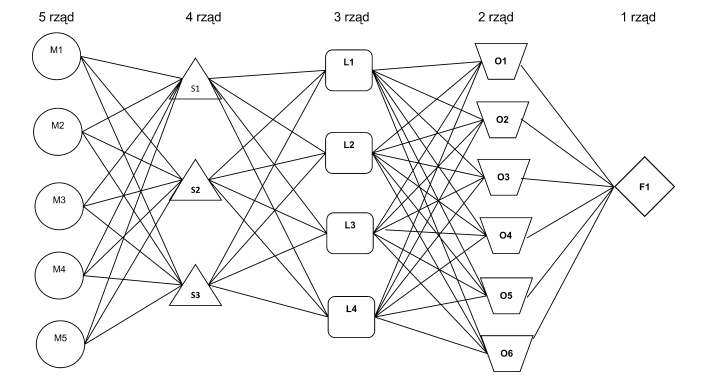
\includegraphics[width=\textwidth]{pictures/siec.png}
  \end{subfigure}
  \captionsetup{margin=10pt,font=small,labelfont=bf,width=.8\textwidth}
  \caption[Przedsiębiorstwo jako graf kierunkowy]{Przedsiębiorstwo przedstawione jako graf kierunkowy. \textit{Źródło:} \cite{Kawa2010}}\label{fig:siecKawa}
\end{figure}
% --- figure --------------------------------------------------------


W niniejszej pracy stosowane jest rozszerzenie tego podejścia, poprzez zaprogramowanie jako agentów jednostek organizacyjnych przedsiębiorstwa \textit{(fabryka, magazyn, sklep, zarząd)}, które razem tworzą system \textit{(przedsiębiorstwo)}. 

To podejście opiera się na obserwacji, że relacje pomiędzy jednostkami w przedsiębiorstwie są analogiczne do relacji uczestników łańcucha dostaw. \cite{Porter1985} zauważył, że działalność przedsiębiorstwa to de facto sekwencja działań, która na każdym ogniwie zwiększa wartość dla odbiorcy. Zasady funkcjononawia opisywanego przez Portera \textit{łańcucha wartości} są identyczne co do opisywanego przez \cite{Moyaux2006} i \cite{Kawa2010} łańcucha dostaw a relacje pomiędzy nimi można przedstawić w sposób zaproponowany przez \cite{Kawa2010} --- z wykorzsystaniem grafu skierowanego, jak zaprezentowano na wykresie \ref{fig:siecKawa}. Podobieństwo to podkreśla fakt, że przedsiębiorstwa poprzez strategię \textit{integracji wertykalnej} swym zasięgiem mogą w rzadkich przypadkach objąć całość łańcucha dostaw.  

Ponieważ przedsiębiorstwa często dysponują wieloma duplikującymi swoje działania jednostkami \footnote{Dobrym przykładem są tutaj zakłady samochodowe, które mogą produkować dany model w różnych krajach. Zmiana fabryki powoduje przy tym radykalną zmianę łańcucha dostaw}, łańcuch ten jest nieliniowy i w jego przypadku mamy do czynienia z podobnymi wyzwaniami co w łańcuchu logistycznym.

Zdefiniowanie jako agentów poszczególnych jednostkek przedsiębiorstwa jest przy tym spójne z określoną przez \cite{Wooldridge1995} charakterystyką agenta, który według ich postulatów posiada : 

	\begin{itemize}
		\item autonomię --- poszczególne jednostki przedsiębiorstwa podążają za strategią i celami narzuconymi przez zarząd, ale mają zazwyczaj swobodę w podejmowaniu decyzji mających na celu ich realizację,
		\item zdolności do komunikacji --- jednostki przedsiębiorstwa komunikują się z otoczeniem (relacje z klientami) oraz między sobą (raportowanie do zarządu, spotkania), a w ramach pomiędzy jednostkami przedsiębiorstwa istnieje asymetria informacji,
		\item reaktywność --- jednostki przedsiębiorstwa reagują na zmiany rynkowe oraz zmiany wewnętrz przedsiębiorstwa,
	 	\item proaktywność --- jednostki przedsiębiorstwa podejmują inicjatywy mające na celu zwiększyć wartość przedsiębiorstwa, jak działalność innowacyjna bądź ekspansja. 
	\end{itemize}
 
 Dlatego w niniejszej pracy będziemy rozważać model wieloagentowy, w którym według założeń na przedsiebiorstwo składać się będzie szereg autonomicznych agentów \textit{(fabryka, magazyn, sklep, zarząd)}, wspólnie tworzących łańcuch dostaw.

\subsubsection{Modelowanie predykcyjne} \label{chapter:statistical} 
W procesach logistycznych i produkcyjnych kluczowym wyzwaniem jest niepewność związana ze zmiennością sprzedaży i jej wartości w chwili $t+1$. Jak wskazuje \cite{James2013} do zmniejszenia niepewności poprzez prognozowanie sprzedaży możemy wykorzystać metody statystyczne. Według \cite{James2013}, zakładając, że dysponujemy zbiorem $n$ obserwacji $p$ zmiennych, możemy zbadać ich relację ze zmienną wyjaśnianą $y$ i otrzymać \textit{model}, który dla nowych - nieanalizowanych wcześniej - obserwacji $x_1,x_2..x_n$  zwraca przewidywaną wartość zmiennej objaśnianej \^{y}. Różnorodne metody modelowania zmiennej objaśnianej (wspólnie nazywane przez \cite{James2013} uczeniem statystycznym, \textit{ang. statistical learning}) mogą być wykorzystane do modelowania predykcyjnego, tj. przewidywania przyszłych wydarzeń na podstawie przeszłej historii danych, w tym również przyszłego wolumenu sprzedaży w przedsiębiorstwie. 

Zastosowanie metod \textit{statistical learning} w przedsiębiorstwach potwierdza \cite{Buckinx2007}, który wskazywał na możliwość prognozowania lojalności klienta na podstawie wewnętrznych danych o transakcjach, oraz \cite{Davenport2011}, który opisuje szereg  \textit{case studies} firm, w których wykorzystuje się istniejące dane o transakcjach do przewidywania przyszłych zakupów klientów. Jednym z podanych przez niego przykładów jest Tesco, które na podstawie zebranych danych przewiduje, jak będzie wyglądał koszyk zakupów klienta podczas następnych zakupów, i odpowiednio wcześnie wysyła mu bony zniżkowe. Również podczas panelu \textit{Strategia B2C w erze Big Data - jak wykorzystać potencjał danych} na XXV Forum Ekonomicznego w Krynicy przedstawicielie polskiego biznesu zwracali uwagę na szerokie wykorzystanie modelowania predykcyjnego również w nasz gospodarce. \footnote{Jednak jak zwracano uwagę, \textit{big data}\ i \textit{modelowanie predykcyjne}\ służą głównie do zyskiwania wiedzy o kliencie i rynku do manualnego przetworzenia analiz , a nie automatyzacji podejmowania decyzji, co rozważamy w tej pracy}

Podane przykłady dają nam podstawy, żeby w przypadku optymalizowanego przedsiębiorstwa zakładać, że dane o każdej transakcji są zapisywane wraz z niektórymi danymi osobowymi klienta \footnote{To stwierdzenie opiera się na opisywanym przez \cite{Davenport2011} przypadku Tesco i zastosowanej przez nich metody zbierania danych. Możliwość zbierania danych o transakcjach określonego klienta daje karta lojalnościowa (lub konto, w przypadku e-commerce), na którą rejestrowana jest każda transakcja. Praktyką jest, żeby przy okazji tworzenia karty lojalnościowej zbierać informacje o kliencie w ankiecie (zakres danych zależy od praktyki korporacyjnej). Dzięki temu, przedsiębiorstwa są w stanie przypisać do zakupów dane osobwe jak płeć, miejsce zamieszkania, wykształcenie etc.}, a cały zbiór danych może być wykorzystany do przewidywania sprzedaży w chwili $t + 1$. 

Dlatego w pracy będziemy zakłądać, że dla każdej transkacji w sklepie dysponujemy zbiorem informacji, zawierące dane o transakcji (\textit{data, miejsce, rodzaj płatności}), produkcie (\textit{nazwa produktu, cena, ilość}) oraz dane osobowe klienta (\textit{płeć, wiek, zarobki, wykształcenie}).

Na podstawie takiego zbioru danych chcemy przewidzieć popyt na produkty w każdym ze sklepów, co w praktyce oznacza konieczność stworzenia modelu estymującego następujące wielkości

	\begin{itemize} 
		\item liczebność poszczególnych grup klientów \footnote{Przez \textit{poszczególne grupy klientów} rozumiemy klientów o wspólnej charakterystyce, czyli takich samych zestawach zmiennych identyfikujących $<kl_1..kl_n>$} odwiedzających sklep w chwili $t+1$,
	\end{itemize}
	oraz, w zależności od zastosowanego podejścia,
	\begin{itemize} 
		\item prawdopodobieństwo z jakim klient o danej charakterystyce kupi produkt,
		\item produkt wybrany przez danego klienta.
	\end{itemize}

Jak wskazuje \cite{James2013}, zmienna objaśniana może przyjąć różne dziedziny --- m.in. zmiennej binarnej (1/0), prawdopodobieństwa, \textit{log odds} lub klasy --- i z tego względu każdy z przypadków różni się metodami które możemy zastosować. Według sugestii \cite{James2013} i \cite{hastie2001} , zastosujemy następujące metody

	\begin{itemize} 
		\item do liczby klientów - regresję metodą OLS (\textit{ordinary least squares, metoda najmniejszych kwadratów})
		\item do prawdopodobieństwa zakupu - regresję logistyczną (\textit{logistic regression})
		\item do wyboru produktu- metody klasyfikacyjne \textit{k-means} oraz \textit{drzewa klasyfikacyjne}
	\end{itemize}
	oraz metody nie służące bezpośrednio do modelowania \^{y}, jednak wspierające proces predykcyjny
	\begin{itemize} 
		\item pomiar odległości (\textit{ang. distance scaling}), poprzez liczenie odległości euklidesowej (\textit{euclidean distance}) pomiędzy dwoma zbiorami danych i stworzenie obliczenie macierzy niepodobieństwa (odległości, \textit{dissmiliarity matrix}
		\item eliminację zmiennych (\textit{ang. backward elimination}), która jest jednym z podejść wyboru podzbiorów (\textit{subset selection}) do selekcji zmiennych wyjaśniających które wspólnie tworzą najlepszy model
		\item prawdopodobieństwo warunkowe do przewidywania, jacy konsumenci odwiedzą sklep w $t+1$.
	\end{itemize}	


\newpage

\subsubsection{Zadanie optymalizacyjne} \label{chapter:zadanie}

Rozważmy przedsiebiorstwo, które za argumentacją przedstawioną w rozdziale \ref{chapter:teoria} oraz obserwacjami  \cite{Moyaux2006} oraz \cite{Kawa2010} przedstawiamy jako system składający się z niezależnych agentów. Zakładamy, że rozważane przedsiębiorstwo składa się z 

\paragraph{Definicja przedsiębiorstwa i grafu}\mbox{}\\

	\begin{itemize} 
		\item zbioru \textit{fabryk} oznaczony przez FA, z generycznym elementem $fa_n \in FA$
		\item zbioru \textit{magazynów} oznaczony przez MA, z generycznym elementem $ma_n \in MA$
		\item zbioru \textit{sklepów} oznaczony przez SK, z generycznym elementem $sk_n \in SK$
		\item \textit{zarządu}, pełniący rolę centralnego koordynatora
	\end{itemize}

Jak zauważył \cite{Kawa2010}, jeśli rozpatrujemy przedsiębiorstwo pod kątem procesów logistycznych możemy zaobserować, że jednostki przedsiębiorstwa będą wspólnie tworzyć graf kierunkowy $S = \{FA \cup MA \cup SK \cup D\}$ (zob. wykres \ref{fig:firma_graf}), gdzie jednostki przedsiębiorstwa $FA, MA, SK$ będą wierzchołkami grafu, a trasy dostaw pomiędzy jednostkami będą krawędziami grafu  $d \in D = \{(i,j) : i \in FA, j \in MA\} \cup \{(i,j) : i \in MA, j \in SK\}$. 

% --- figure --------------------------------------------------------
\begin{figure}[hbt]
  \centering
\begin{center}
\begin{tikzpicture}
   % Draw all levels
  \draw[level] (0,0) -- node[above] {fabryka  $fa_1$} node[below] {($k_{fa_1}$)}  (2,0);
  \draw[connect] (2,0)  -- (3,-1);
  \draw[connect] (2,0) -- (3,1);
  \draw[connect] (2.5,0.75) -- (2.5,0.75) node[below] {$d_1$};
  \draw[connect] (2.5,-0.75) -- (2.5,-0.75) node[below] {$d_2$};
  \draw[level]   (3,1)  -- node[above] {magazyn  $ma_1$} node[below] {($k_{ma_1}$)} (5,1);
  \draw[level]   (3,-1) -- node[above] {magazyn $ma_2$} node[below] {($k_{ma_2}$)} (5,-1);
  \draw[connect] (5,1)    -- (6,2) (5,1) -- (6,0) (5,1) -- (6,-2) (5,1);
  \draw[connect] (5,-1)    -- (6,2) (5,-1) -- (6,0) (5,-1) -- (6,-2) (5,-1);
  \draw[level]   (6,2)  -- node[above] {sklep $sk_1$} node[below] {($k_{sk_1}$)}  (8,2); 
  \draw[level]   (6,-2)  -- node[above] {sklep $sk_2$}node[below] {($k_{sk_1}$)}  (8,-2);
  \draw[level]   (6,0)  -- node[above] {sklep $sk_3$}node[below] {($k_{sk_1}$)}  (8,0);
  \node[text width=5cm] at (11,2.5) {  $ w_1 = {fa_1,ma_1,sk_1, d_1,d_3}  $};
  \node[text width=5cm] at (11,1.5) {  $ w_2 = {fa_1,ma_1,sk_2, d_1,d_4}  $};
  \node[text width=5cm] at (11,0.5) {  $ w_3 = {fa_1,ma_1,sk_3, d_1,d_5}  $};
  \node[text width=5cm] at (11,-0.5) {  $ w_4 = {fa_1,ma_2,sk_1, d_2,d_6}  $};
  \node[text width=5cm] at (11,-1.5) {  $ w_5 = {fa_1,ma_2,sk_2, d_2,d_7}  $};
  \node[text width=5cm] at (11,-2.5) {  $ w_6 = {fa_1,ma_2,sk_3, d_2,d_3}  $};
  % Draw labels
  \node[label] at (1,3.5)  {\textit{Fabryki}};
  \node[label] at (4,3.5)  {\textit{Magazyny}};
  \node[label] at (7.5,3.5)  {\textit{Sklepy}};
  \node[label] at (10.75,3.5)  {\textit{Ścieżki}};
  % Draw annotations
\end{tikzpicture}
\end{center}
  \captionsetup{margin=10pt,font=small,labelfont=bf,width=.8\textwidth}
  \caption[Rozważane przedsiębiorstwo przedstawione jako graf kierunkowy]{Rozważane przedsiębiorstwo przedstawione jako graf kierunkowy. \textit{Źródło:} opracowanie własne}\label{fig:firma_graf}
\end{figure}
% --- figure --------------------------------------------------------

Planowanie produkcyjno-logistyczne w przedsiębiorstwie będzie polegało na alokacji wolumenów produkcji na poszczególne ścieżki $w \in W = {(fa,ma,sk,d_1,d_2)} $ \footnote{Ścieżka zawiera dwa elementy ze zbioru krawędzi $d$, ponieważ zawiera krawędź \textit(fabryka --- magazyn) oraz \textit(magazyn --- sklep)}. 

Należy zaznaczyć, że optymalizacja alokacji ścieżek zamiast krawędzi ma znaczenie praktyczne dla przedsiębiorstw, szczególnie międzynarodowych. Dzisiejsze trendy globalizacyjne spowodowały, że często produkcja w danym kraju trafia na wiele rynków, a każda z partii musi być dostosowana do rynków lokalnych \footnote{Ze względów zarówno regulacyjny, jak i preferencji klientów. Dodatkowo, w niektórych branżach, jak samochodowej, można dostosowywać specyfikację zamawianego produktu. W takim przypadku również należy zapewnić, że trafi on do miejsca docelowego} --- czyli w momencie produkcji produkt musi mieć określone miejsce docelowej dostawy. W logice grafu oznacza to, że przedsiębiorstwo musi określić ruch na całej ścieżce produktu, nie tylko do następnej krawędzi.   

\paragraph{Równanie zysku przedsiębiorstwo}\mbox{}\\

W tak zdefiniowanym grafie proces logistyczny odbywa się przepływem wdłuż krawędzi $D$, a z każdym z elementów grafu $S$ zwiążany jest koszt przepływu $k_ j = f_j(x_j)$ \footnote{Warto zauważyć, że koszt przesyłu nie oznacza tylko kosztów transportu, ale także kosztów produkcji w fabryce, kosztów magazynowania oraz kosztów obsługi procesów sprzedaży w sklepie, tak więc koszt ten będzie definiowany nie tylko na krawędziach $D$, ale każdym elemencie grafu $S$}, gdzie $f$ jest dowolną funkcją kosztu, $j$ rozważanym elementem grafu $S$, a $x_j$ wolumenem produkcji przechodzącym przez dany element. 

Sprzedaż towarów przepływających przez graf następuje w sklepach, a zakładajac, że przedsiebiorstwo nie stosuje dyskryminacji cenowej, cena produktu będzie globalna i stała \footnote{Rozumiemy przez to, że cena jest identyczna dla wszystkich klientów, dla wszystkich sklepów oraz wszystkich okresów czasu $t$}. Przychód $r$ w każdym ze sklepów $sk \in SK$ przy cenie $p$ będzie równy $r = p \times q_{sk}$, gdzie $q$ to sprzedaż w wybranym sklepie $sk$ \footnote{Warto zauważyć, że sprzedaż $q_j$ nie jest tym samym co wolumen $n_j$, ponieważ dostarczenie towaru do sklepu nie gwarantuje jego sprzedaży}. 

Dla całego systemu funkcja zysku systemu $P_s$ będzie zależała przede wszystkim od alokacji wolumenów zadany równaniem \ref{eq:zysk} 

\begin{equation} \label{eq:zysk}
P = \sum\limits_{sk} p \times q_{sk} - \sum\limits_{j} f_j(x_j)
\end{equation}

\begin{center} gdzie $p$ to stała cena, \\ $q_{sk}$ to sprzedaż w sklepie $sk \in SK$ spełniająca warunek $q_{sk} \le x_{sk}$ \\ a $f_j$ to dowolna funkcja kosztu zależna od wolumenu $x_j$ w elemencie grafu $j \in S$ \end{center}

To zadanie optymalizacyjne byłoby względnie proste \footnote{Pomijając aspekt złożoności obliczeniowej}, gdybyśmy mieli doskonałą informację na temat poziomu sprzedaży w każdym ze sklepów w chwili $ t + 1 $. Na taką wiedzę nie możemy liczyć ani w tej pracy, ani w w rzeczywistości, dlatego rozwiązaniem proponowanym w niniejszej pracy jest zastosowanie modelowania predykcyjnego (\textit{predictive analytics}), w celu prognozowania liczby klientów i ich wyborów w każdym ze sklepów w najbliższych okresach czasu. \footnote{Obecnie w przedsiębiorstwach rzadko stosuje się zaawansowane sposoby prognozowania sprzedaży (\textit{predictive analytics}), a zarządzanie dostawami odbywa się raczej metodą manualnego uzupełniania zapasów.} 

Ponadto, jak warto zauważyć, nie możemy liczyć na to, że funkcja kosztu $f_j$ będzie liniowa. Wspominana przez \cite{Kawa2010} maksymalna przepustowość każdego z łańcuchów, która w przedsiębiorstwie będzie spowodowana ograniczonymi mocami produkcyjnymi, może spowodować, że funkcja kosztu będzie dowolną funkcją, co empirycznie potwierdzone jest w powszechności efektów skali w każdym z sektorów gospodarki. Warto przy tym zauważyć, że efekty skali mogą być zarówno dodatnie, jak i ujemne, jak również ich wspólne występowanie \footnote{Dodatnie gdy produkcja będzie mniejsza niż optymalny poziom produkcji, a ujemne po przekroczeniu optymalnych mocy produkcyjnych}.

Trzecim aspektem który trzeba wziąć pod uwagę jest złożoność obliczeniowa. Nawet dla prostego układu, lecz wolumenu produkcji ponad 1000 sztuk sprawdzenie zysku w przypadku wszystkich kombinacji alokacji wymaga olbrzymiej ilości iteracji. Mimo znaczącego wzrostu mocy komputerów w ostatnich latach, wolumeny produkcji w dużych przedsiębiorstwach oraz złożoność tras logistycznych sprawia, że to podejście jest kompletnie niepraktyczne i należy szukać alternatywnych podejść, upraszczających problem.

 Proponowany algorytm będzie brał wszystkie te aspekty pod uwagę, a pierwszy z wymienionych problemów rozwiążemy wykorzystując  \textit{modelowanie predykcyjne}.

\subsection{Proponowany algorytm optymalizacyjny} \label{chapter:algorytm}

W proponowanym algorytmie optymalizacyjnym wykorzystujemy fakt, że dzięki modelowaniu predyktywnemu możemy prognozować wolumen sprzedaży $q_{sk}$ w każdym ze sklepów $sk \in SK$. Ponieważ równolegle zakładamy brak stosowania dyskryminacji cenowej, część przychodowa równania \ref{eq:zysk} będzie nam znana, i możemy ją oznaczyć jako stałą $r_s$, oznaczającą  przychód całego systemu.  

\begin{equation} \label{eq:przychodsystemu}
P_s = r_s - \sum\limits_{j} f_j(x_j)
\end{equation}

Ponieważ w rozdziale \ref{chapter:zadanie} stwierdziliśmy, że ze względów biznesowych naszym celem jest optymalizacja alokacji wolumenu na ścieżkach, zauważmy, że $x_j$ będzie równe $\sum\limits_{w:j \in w} x_w$, sumie wolumenów $x_w$ na wszystkich ścieżkach $w \in W$ przechodzących przez element grafu $j \in S$, dzięki czemu równanie \label{eq:przychodsystemu} możemy zapisać jako: 

\begin{equation} \label{eq:przychodsystemu}
P_s = r_s - \sum\limits_{j} f_j(\sum\limits_{w:j \in w} x_w)
\end{equation}

Dzięki temu przekształceniu możemy wyznaczyć gradient funkcji zysku...

\begin{equation} \label{eq:gradient}
\bigtriangledown P_s  = [\frac{\partial P_s}{\partial x_{w_1}}...\frac{\partial P_s}{\partial x_{w_n}}]
\end{equation}
\begin{center} gdzie $P_s$ to funkcja zysku, $X_w$ to wolumen przechodzący przez ścieżkę $w \in W$, \\ a $n$ to ilość ścieżek w zbiorze $W$ \end{center}

... który wskaże nam kierunek najszybszych wzrostów wartości funkcji zysku $P_s$ w zależności od ulokowania kolejnego produktu na którejś ze ścieżek. Zakładajac, że działanie algorytmu zaczyna się, gdy każda ze ścieżek $w \in W$ jest pusta, tj. każde $x_{w}=0$, działanie algorytmu jest następujące

\begin{enumerate} 
	\item wyznacz gradient funkcji zysku $P_s$
	\item stwórz wektor $A$ wszystkich ścieżek $w \in W$, który będzie nam służył do iterowania pętli 
	\item dla każdego produktu lub partii produktu oblicz gradient w punkcie $[x_{w_1}, x_{w_n}]$. 
	\item dla każdego elementu wektora $A$ sprawdź, 
		\begin{itemize}
			\item czy odpowiadająca mu wartość pochodnej cząstkowej jest mniejsza od 0
			\item czy dodanie kolejnego produktu do ścieżki spowoduje, że w sklepie leżącym na ścieżce przestanie być spełniany warunek $q_{sk} \le x_{sk}$ \footnote{Wolumen dostaw będzie większy niż prognozowany wolumen sprzedaży} 
		\end{itemize}
	\item jeśli którykolwiek z powyższych jest prawdą, usuń ścieżkę z wektora $A$
	\item jeśli wektor $A$ nie jest pusty, z pozostałych elementów wektora $A$, wybierz ścieżkę o największej wartości pochodnej cząstkowej w gradiencie
	\item powtórz od kroku 3. dopóki wektor $A$ nie będzie pusty.
\end{enumerate}

Działanie algorytmu w standarcie UML zaprezentowane zostało na wykresie \ref{fig:algorytm}.

\begin{figure}
  \centering
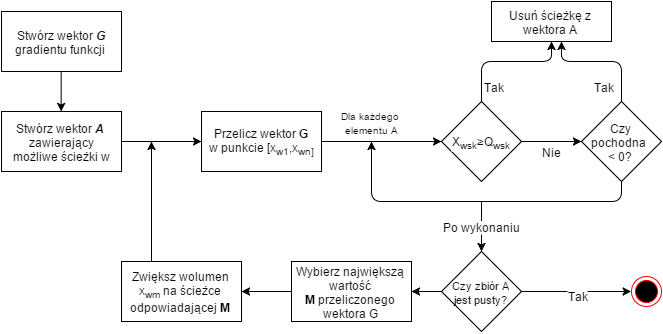
\includegraphics[width=\linewidth]{pictures/diagramoptymalizacyny.png}
  \caption{Proponowany algorytm optymalizacyjny}
  \label{fig:diagramoptymalizacyny}

\end{figure}

\subsection{Cechy algorytmu optymalizacyjnego}

Algorytm działający według reguł opisanych w rozdziale \ref{chapter:algorytm} będzie heurystyką, ponieważ kierując się najszybszymi wzrostami w punkcie obliczania gradientu może ominąć maksimum globalne. Gwarantuje za to znalezienie maksimum lokalnego i zakończenie pętli \footnote{Tj. nie ma możliwości, żeby iterował w nieskończoność}. Biorąc pod uwagę, że w aspekcie praktycznym większość funkcji kosztów nie będzie miało nietypowych wzorów, algorytm też powinien być w zupełności wystarczający do większości zastosowań optymalizacyjnych.

Ponieważ algorytm nie oblicza wszystkich możliwych kombinacji alokacji wolumenów, a używa gradientu do oszacowania najbardziej opłacalnej trasy dla każdego z produktów, czas jego wykonania będzie znacznie krótszy w stosunku do algorytmu kompletnego. Liczba iteracji potrzebnych do kalkulacja zysku w przypadku każdej możliwej kombinacji alokacji będzie liczbą Stirlinga II rodzaju, a w przypadku algorytmu maksymalna liczba iteracji będzie iloczynem liczby produktów oraz liczby ścieżek. \footnote{W praktyce będzie mniejsza, ponieważ algorytm pozbywa się nierentownych i zapełnionych ścieżek}. 

Warto zauważyć, że w sytuacji, gdy skala działalności firmy powoduje, że graf jest bardzo rozbudowany, sposób działania algorytmu pozwala predefiniować w macierzy $A$ najbardziej prawdopodobne trasy. Pozwoli to zmniejszyć liczbę iteracji, jednocześnie zachowując integralność grafu - inne metody wymagałyby zmiany jego struktury.

Innym ograniczeniem algorytmu jest to, że szukając kolejnych optymalnych punktów "porusza się" on dyskretnie po wykresie funkcji. Wynika to z założenia, że w procesach logistycznych nie możemy przekroić i przetransportować pół produktu, a nawet ładunek drobnicowy będzie miał swoją jednostkę najmniejszego możliwego transportu, jak paleta, tona, kontener etc. 

% --- chapter ---------------------------------------------------------
\clearpage

\section{Model} \label{chapter:model}

W celu sprawdzenia działania algorytmu zbudowany został model wieloagentowy, który symuluje lokalny rynek na wybrany produkt, wraz z zachowaniami konsumentów i funkcjonowaniem przedsiębiorstwa.

\subsection{Koncepcja modelu} \label{chapter:koncepcja}

Zgodnie z argumentacją zawartą w rozdziale \ref{chapter:teoria}, relacje w przedsiębiorstwie pomiędzy jednostkami tworzącymi wspólnie łańcuch dostaw można przedstawić jako model wieloagentowy. Jednocześnie, inspirując się \cite{Kaminski2012}, zakładamy, że możemy stworzyć heteregenicznych agentów oraz symulować ich decyzje celu modelowania zachowań i trendów na rynku. 

Łącząc te podejścia, celem pracy jest stworzenie modelu wieloagentowe symulującego rynek (w szczególności kładąc nacisk na aspekt sprzedaży oraz dostaw) na którym moglibyśmy sprawdzić wpływ działania algorytmu na wyniki przedsiębiorstwa.

Zgodnie z powyższym, w modelu znajdą się następujący typy agentów: 

\begin{itemize} 
	\item \textbf{klienci}, który zgodnie z założeniem będą heterogeniczni i definiowani przez cechy demograficzne \footnote{Są to między innymi wiek, zarobki, wykształcenie, zainteresowania - zostanie to dokładnie opisane w dalszej części pracy.}, które wpływającą na podejmowane przez niego decyzje oraz zachowania, 
	\item \textbf{przedsiębiorstwo}, sprzedające \textit{produkt} na rynku. Zgodnie z podejściem przedstawionym w \ref{chapter:teoria}, przedsiębiorstwo będzie rozumiane jako zbiór niezależnych, współpracujących ze sobą agentów 
		\begin{itemize}
			\item fabryk
			\item magazynów
			\item sklepów 
			\item oraz zarządu, pełniącego funkcje koordynującą 
		\end{itemize}
	\item \textbf{konkurencji}, zachowującej się pasywnie w stosunku do rynku, konsumentów i symulowanego przedsiębiorstwa, ale wprowadzajacej na rynek szereg produktów stanowiących alternatywę dla produktu symulowanej firmy \footnote{Tj. konkurencja nie zmienia decyzji podjętych przed rozpoczęciem gry, i w założeniu ma stanowić jedynie alternatywę dla konsumentów.} 
	\item \textbf{produktów} dostępnych na rynku, z których każdy zdefiniowany jest unikalnymi cechami określającymi jakość, typ i cenę produktu, przez co każdy z produktów będzie preferowany przez inną grupę konsumentów, a preferencje są oparte na danych ze świata rzeczywistego. 
\end{itemize}

\paragraph{Aspekt lokalizacji}\mbox{}\\

Aby dobrze odwzorować kluczowy aspekt lokalizacji i dróg w łańcuchach dostaw, symulowany rynek jest osadzony w \textit{wirtualnym mieście}. Oznacza to, że każdy agent ma swoją lokalizację w macierzy o wymiarach $x \times y$ i może się w niej poruszać po wyznaczonych drogach.

Lokalizacja wpływa na działania agenta - klient kupi produkt tylko w sklepie który będzie na jego ścieżce, a dostawa z magazynu do sklepu będzie tym droższa, im bardziej oddalone będą od siebie. 

\paragraph{Symulowanie decyzji konsumenckich}\mbox{}\\

W modelu konsumenci nieustannie poruszają się po \textit{mapie}, bez związku z działaniem przedsiębiorstwa \footnote{Ruchy są wywołane przez losowe zdarzenia którym może być poddany konsument. Zdarzenia wymagają od niego podróży do jednego z predefiniowanych miejsc --- jak praca czy dom innego agenta}. W każdej jednostce czasu $ t $ klienci z prawdopodobieństwem $ p $ będą potrzebować symulowany produkt. Wywołanie tego zdarzenia spowoduje, że podczas losowej podróży z punktu A do B odwiedzą oni losowy sklep z wszystkich sąsiadujących z trasą, a następnie wybiorą jeden z produktów dostępnych w sklepie \footnote{Sklepy nie przynależą do przedsiębiorstwa, więc znajdują się tam także produkty konkurencji, i spośród wszystkich klient dokonuje wyboru.}. 

Symulacja wyboru opiera się na danych o preferencjach konsumenckich zebranych w grze ekonomicznej na próbie 169 badanych, w wyniku których otrzymano 1860 rekordów danych \footnote{Gra ekonomiczna została dokładniej opisana w rozdziale \ref{chapter:customerresearch}}. Na ich podstawie których zbudowane zostało drzewo klasyfikacyjne opisujące prawdopodobieństwo zakupu produktu od cech konsumenta. 

Ponieważ każdy konsument-agent w modelu ma swoje unikalne cechy demograficzne i charakteru, spójne z danymi zebranymi w ankiecie, wykorzystujemy zbudowane drzewo klasyfikacyjnego do określenia wyboru, jakiego najprawdopodobniej w świecie rzeczywistym dokonał by jego odpowiednik, posiadający identyczne bądź zbliżone cechy. \footnote{Oczywiście, o wiele lepsze byłoby oparcie pracy o prawdziwe historie transakcji, jednak jest to niemożliwe ze względu na dużą poufność tych danych} Przeprowadzając podobny proces dla każdego konsumenta w modelu, otrzymujemy dynamiczną symulację rynku produktów szybkozbywalnych. 

\paragraph{Decyzje przedsiębiorstwa}\mbox{}\\

Ponieważ, jak zostało wspomniane, konsument wybiera produkt tylko z gamy dostępnych w sklepie, kluczowe dla sukcesu przedsiębiorstwa w modelu jest dostarczenie w każdej jednostce czasu $t$ odpowiedniej ilości produktów \footnote{W warunkach symulacji nie można zapełnić \textit{półek sklepowych} do pełna, bo brak sprzedaży oznacza stratę dla przedsiębiorstwa, a w sektorze FMCG zakładamy, że w czasie $t+1$ produkty stracą zdolność do spożycia}. Oznacza to, że przed rozpoczęciem każdej tury przedsiębiorstwo musi podjąć szereg decyzji o m.in.

	\begin{itemize}
		\item odpowiednim poziomie produkcji,
		\item wolumenie dostaw do każdego ze sklepów w sieci,
		\item rozdzieleniu wolumenów pomiędzy jednostki przedsiębiorstwa, tj. ile z całkowitego wolumenu ma wyprodukować fabryka $A$, a ile fabryka $B$
	 	\item ścieżki jakimi powinny zostać wysłane dostawy do każdego ze sklepów. \footnote{Rozumiemy przez to pytanie, który z magazynów ma być pośrednikiem, ponieważ dobra nie mogą być dostarczane bezpośrednio z fabryki do sklepu.}
	\end{itemize}

Każda z tych decyzji będzie miała wpływ na przychody \footnote{Przy założeniu stałej ceny, będą to przede wszystkim \textit{utracone koszty} w przypadku wyczerpania się zapasów w sklepie} oraz koszty firmy. W modelu przedsiębiorstwo przez $n$ jednostek czasu $t$ przedsiębiorstwo korzysta z predefiniowanych zasad podejmowania decyzji, które oparte są na najczęstszych praktykach spotykanych w świecie rzeczywistym: 

	\begin{itemize}
		\item towar zamawiamy jest zawsze z najbliższego magazynu
		\item ilość zamówionego towaru do każdego ze sklepów równa jest sprzedaży $t_0$ \footnote{Gdzie $t_0$ to runda próbna, która ma na celu sprawdzenie popytu na rynku i nie jest zapisywana do wyników firmy. Jej wdrożenie ma na celu odwzierciedlenie w modelu wiedzy powszechnej o rynku, tj. przedsiębiorcy wiedzą ile mogą sprzedać na podstawie tego, co sprzedawali w niedalekiej przeszłości albo na podstawie raportów rynkowych}
	\end{itemize}

Po $n$ rund, przez pozostałą ilość okresów $t$ decyzje w przedsiębiorstwie podejmowane są na podstawie algorytmu optymalizującego, opisanego w rozdziale \ref{chapter:algorithm}. 

\subsection{Zastosowane narzędzia}

Model został zbudowany w języku programowania Python 2.7, z wykorzystaniem następujących bibliotek (zob.tabela \ref{tab:biblioteki}) : 

% --- figure --------------------------------------------------------
\begin{table}[hbt]
  \centering
  \captionsetup{margin=10pt,font=small,labelfont=bf,width=.8\textwidth}
  \caption[Zastosowane biblioteki języka Python]{Zastosowane biblioteki języka Python. \textit{Źródło:} opracowanie własne.}
  \label{tab:biblioteki}
\vspace*{2ex}
  \begin{tabular}{lccc}
 Biblioteka & Źródło & Zastosowanie \\ 
\hline
 Sympy & www.sympy.org & Wykorzystanie do obliczeń symbolicznych \\  
 scikit-learn & scikit-learn.org & Wykorzystanie bibliotek metod statystycznych \\ \hline
  \end{tabular}
\end{table}
% --- figure --------------------------------------------------------


Kod programu dostępny jest pod adresem  \textit{github.com/hubertguzera/master-thesis}

\subsection{Struktura programu}

Program podzielony jest na trzy moduły, jak zaprezentowano na rysunku \ref{fig:struktura}

	\begin{itemize}
		\item Pierwsza odpowiada za stworzenie, w drodze losowań, środowiska w ramach którego toczy się symulacja, wraz z agentami i macierzą lokalizacji. \footnote{Model może pominąć tą część i wczytać pregenerowany świat w celu sprawdzenia różnych scenariuszy w statycznym świecie (ceteris paribus).}
		\item  Druga część przez $t_n$ jednostek czasu symuluje działanie rynku --- decyzji klientów i funkcjonowania przedsiębiorstwa --- według predefiniowanych zasad sterowań \footnote{Co istotne, algorytm optymalizacyjny jeszcze nie jest implementowany na tym etapie}, zwracając na koniec wyniki (przychody, koszty i zysk) przedsiębiorstwa w danej jednostce czasu $t$.
		\item Trzecia po $t_n$ rund symulacji aplikuje algorytm optymalizacyjny, który poprzez prognozowanie sprzedaży na krańcach grafu w $t_{n+1}$, szuka najlepszych decyzji o alokacji produktów. Działanie algorytmu można porównać do miary porównawczej uzyskanej w pkt 2. 
	\end{itemize}


% --- figure --------------------------------------------------------
\begin{figure}[hbt]
  \centering
  \begin{subfigure}[t]{0.95\textwidth}
    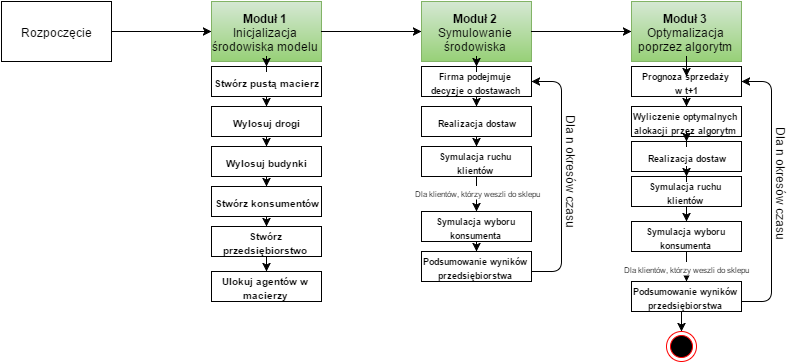
\includegraphics[width=\textwidth]{pictures/Struktura.png}
  \end{subfigure}
  \captionsetup{margin=10pt,font=small,labelfont=bf,width=.8\textwidth}
  \caption[Struktura działania programu]{Struktura działania programu \textit{Źródło:} opracowanie własne}\label{fig:xxx1}
\end{figure}
% --- figure --------------------------------------------------------


\subsection{Generowanie środowiska modelu}
\paragraph{Klasa \textit{rynek}}\mbox{}\\
Za reprezentację tak opisanego środowiska modelu odpowiada klasa \textit{rynek}, wobec której dziedziczą wszystkie inne klasy występujące w modelu. Klasa \textit{rynek} (i wszystkie dziedziczące) jest generowana dynamicznie i losowo \footnote{Jednak może być zapisana jeśli istnieje konieczność replikacji obliczeń albo porównań.}.  Konstrukcja klasy \textit{rynek} w programie została zaprezentowana w diagramie \ref{UML:rynek}. \\


% --- figure --------------------------------------------------------
\begin{figure}[hbt]
  \centering
\begin{tikzpicture} \label{rynek}
\begin{class}[text width=11cm]{rynek}{0,0}
\attribute{swiat : class}
\attribute{symulowana\_firma : class}
\attribute{tura : integer}
\attribute{produkty\_na\_rynku : class}
\operation{\_\_init\_\_(self,swiat) : None}
\operation{sprzedaz\_w\_sklepach(self) : None}
\operation{nowatura (self) : None}
\end{class}
\end{tikzpicture}
  \captionsetup{margin=10pt,font=small,labelfont=bf,width=.8\textwidth}
  \caption[Diagram UML klasy rynek]{Diagram UML klasy rynek \textit{Źródło:} opracowanie własne}\label{UML:rynek}
\end{figure}
% --- figure --------------------------------------------------------


\paragraph{Klasa \textit{świat}}\mbox{}\\

Klasa \textit{swiat} zawarta w klasie \textit{rynek} i zaprezentowana na diagramie \ref{UML:swiat} powstała w celu odpowiedniego odwzorowania kluczowego aspektu lokalizacji i dróg w łańcuchach dostaw, wzorując się na podejściu zastosowanym w \textit{modelu segregacji Schellinga} (\cite{Schelling1971}). Agenci osadzoni są w przestrzeni, reprezentowaną przez macierz klas \textit{lokalizacja} o wymiarach (x,y). Dodatkowo, lokalizacje są połączone drogami, wymusząjąc na agentach poruszanie się tylko w obrębie ścieżek. Dzięki temu, w modelu będziemy mogli wiernie odwzorować wpływ odległości i wyboru trasy na efektywność procesów logistycznych, oraz zależność wyników sklepu od zamieszkującej okolicę populacji. 

Macierz \textit{mapa} generowana jest generowana jest według algorytmu widocznego na rysunku \ref{fig:lokalizacje}, który gwarantuje następujące właściwości otrzymanej w ten sposób macierzy lokalizacji. 

	\begin{itemize}
		\item Drogi krzyżują się i skręcają tylko pod kątem prostym. Poza skrzyżowaniami, drogi nie mają w sąsiedztwie innych dróg,
		\item Inne lokalizacje (domy, sklepy etc.) mogą występować tylko w bezpośrednim sąsiedztwie drogi,
		\item Drogi stanowią ciągłą linię, dzięki czemu nie ma punktu, do którego nie dałoby się dojechać z dowolnego miejsca startowego,
		\item W regione 2 punktów od skraju mapy nie są generowane ani drogi, ani lokalizacje.  \footnote{Jest to zabezpieczenie algorytmu, który w odległości 2 pkt od skraju mapy ma 0 proc. szansy na poprowadzenie ścieżki dalej - ponieważ w przypadku iterowania na skrajach mapy niektóre funkcje (jak sprawdzenie sąsiadujących punktów) mogą odnieść się do lokalizacji poza macierzą, powodując błąd programu}
	 	\item Gęstość sieci dróg oraz prawdopodobieństwo występowania zakrętów jest predefiniowana przez użytkownika
	\end{itemize}

Przykładowa \textit{mapa} otrzymana w wyniku działania algorytmu widoczna jest na rysunku \ref{fig:mapa}.
 \\

% --- figure --------------------------------------------------------
\begin{figure}[hbt]
  \centering
\begin{tikzpicture}
\begin{class}[text width=11cm]{swiat}{-1,0}
\attribute{mapa : array \textit{--- macierz lokalizacji o wymiarach x,y}}
\attribute{ludnosc : array type \textit{--- macierz instacj klasy konsument}}
\attribute{ludnosc : dictionary \textit{--- slownik sieci drog}}
\end{class}
\begin{class}[text width=7cm]{lokalizacja}{-5,-5}
\inherit{swiat}
\attribute{typ : string \textit{--- typ budynkui}}
\attribute{x : integer \textit{--- lokalizacja x}}
\attribute{y : integer  \textit{--- lokalizacja y}}
\attribute{droga : array \textit{--- przylegla droga}}
\end{class}
\begin{class}[text width=7cm]{konsument}{3,-5}
\inherit{swiat}
\attribute{plec : string}
\attribute{wiek : integer}
\attribute{zarobki : integer}
\attribute{zainteresowania : array}
\attribute{wyksztalcenie : integer}
\attribute{okazja : boolean}
\attribute{domx : integer}
\attribute{domy : integer}
\attribute{pracax : integer}
\attribute{pracay : integer}
\operation{odwiedzony\_sklep(self,swiat) : None}
\operation{macierz\_cech(self) : array}
\end{class}
\end{tikzpicture}
  \captionsetup{margin=10pt,font=small,labelfont=bf,width=.8\textwidth}
  \caption[Diagram UML klasy swiat, lokalizacja i konsument]{Diagram UML klasy swiat, lokalizacja i konsument \textit{Źródło:} opracowanie własne}\label{UML:swiat}
\end{figure}
\begin{figure}[hbt]
  \centering
  \begin{subfigure}[t]{1\textwidth}
    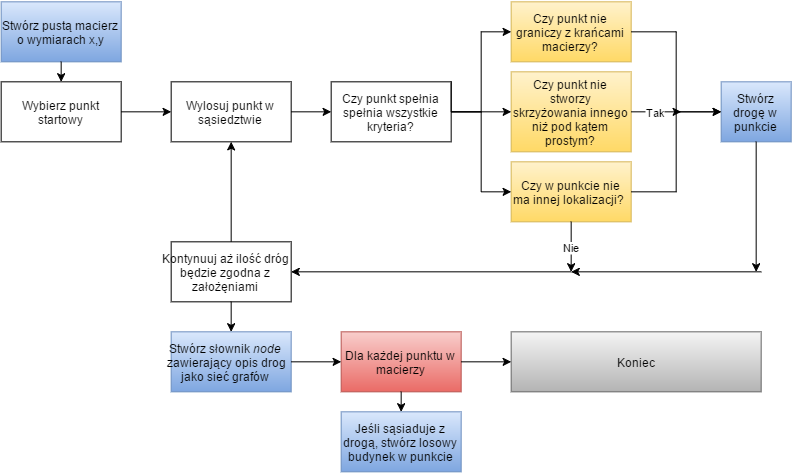
\includegraphics[width=\textwidth]{pictures/tworzeniedrog.png}
  \end{subfigure}
  \captionsetup{margin=10pt,font=small,labelfont=bf,width=.8\textwidth}
  \caption[Algorytm generowania świata w modelu]{Algorytm generowania świata w modelu. \textit{Źródło:} opracowanie własne}\label{fig:lokalizacje}
\end{figure}
% --- figure --------------------------------------------------------
% --- figure --------------------------------------------------------
\begin{figure}[hbt]
  \centering
  \begin{subfigure}[t]{0.45\textwidth}
    
\includegraphics[width=\textwidth]{../mapy/po_lokalizacji_sklepow.png}
  \end{subfigure}
  \captionsetup{margin=10pt,font=small,labelfont=bf,width=.8\textwidth}
  \caption[Przykładowa wygenerowana mapa]{Przykładowa mapa - \textit{szary} to drogi, \textit{niebieski} - domy mieszkalne, \textit{czerwony} i \textit{zielony} - biurowce, \textit{pomarańczowy} - sklepy, \textit{żółty} - magazyny, \textit{błękitny} - fabryki \textit{Źródło:} opracowanie własne}\label{fig:mapa}
\end{figure}
% --- figure --------------------------------------------------------


\subsubsection{Algorytm wyszukiwania drogi} 

Trasy pomiędzy zadanymi punktami w modelu są wyszukiwane dynamicznie, na podstawie algorytmu wyszukiwania drogi. Odległości z kolei obliczane są poprzez sumowanie ilości punktów w zwracanym przez algorytm łańcuchu. 

Algorytm oparty jest na metodach wyszukiwania ścieżek w grafach, dzięki założeniu, że każda droga o współrzędnej (x,y) na mapie jest punktem grafu, który może sąsiadować z punktami o współrzędnych (x-1,y),(x+1,y),(x,y+1),(x,y-1) \footnote{Punkty (x-1,y-1),(x+1,y-1),(x+1,y+1),(x-1,y+1) wykluczamy przez wcześniejsze założenie, że drogi krzyżują się tylko pod katem prostym}, o ile również są drogrami. \footnote{Informacje o punktach i sąsiadujących przechowywane są w zmiennej nodes, która jesst słownikiem, dla każdego klucza - punktu na mapie - przechowuje informacje o sąsiadujących punktach, np. (3,2) = [(3,3)(4,3)].} \footnote{Pewnym ograniczeniem jest, że jako punkty grafu definiujemy tylko drogi, tak więc szukając trasy z punktu A do punktu B de facto szukamy trasy z drogi przy punkcie A do drogi przy punkcie B.}

Algorytm, udostępniony przez Python Foundation \footnote{https://www.python.org/doc/essays/graphs/} i zaprezentowany w tabeli \ref{fig:wayfinding} ma następujące cechy
	\begin{itemize}
		\item jest rekurencyjny,
		\item nie jest losowy,
		\item nie gwarantuje znalezienia najkrótszej trasy.
	\end{itemize}


% --- figure --------------------------------------------------------
\begin{figure}[hbt]
  \centering
\begin{lstlisting}[frame=single, label=szukaniedrogi]  
    def find_path(graph, start, end, path=[]):
        path = path + [start]
        if start == end:
            return path
        if not graph.has_key(start):
            return None
        for node in graph[start]:
            if node not in path:
                newpath = find_path(graph, node, end, path)
                if newpath: return newpath
        return None
\end{lstlisting}
  \captionsetup{margin=10pt,font=small,labelfont=bf,width=.8\textwidth}
  \caption[Algorytm wyszukiwania drogi]{Algorytm wyszukiwania drogi\textit{Źródło:} opracowanie własne}\label{fig:konsument}
\end{figure}
% --- figure --------------------------------------------------------


\subsection{Agenci, ich rodzaje i właściwości}
\subsubsection{Konsumenci} \label{chapter:konsumenci}

Idąc za \cite{Kaminski2012}, w modelu stosujemy modelowanie rynku za pomocą heterogeniczne konsumentów. Stąd, każdy z konsumentów ma swoją unikalną charakterystykę rozumianą przez cechy demograficzne oraz cechy charakteru, które będą wpływać na jego wybory. 

W dodatku, chociaż agenci nieustannie poruszają się w ramach modelu, to pula lokalizacji w ramach których będą się przemieszczać jest ograniczona. Każdy z konsumentów będzie się przemieszczał tylko w wyniku predefiniowanych zdarzeń, których liczba dla każdego konsumenta jest ograniczona do czterech \footnote{Warto zauważyć, że każde ze zdarzeń wywołuje przemieszczenie do korespondującej lokalizacji, tak zdarzenie będzie zawsze wywoływać podróże tej samej lokacji}, tak więc agent będzie przemieszczał się pomiędzy maksymalnie czterami lokalizacjami, tworząc pewne wzorce zachowań. 

Dzięki temu, odwzierciedlamy zjawisko ze świata rzeczywistego, że konsumenci zazwyczaj robią zakupy w ograniczonej liczbie sklepów będących po drodze bądz niedaleko. Jest to bardzo istotny warunek funkcjonowania modelu, ponieważ losowy dobór klientów uniemożliwiłby modelowanie predykcyjne.

Każdy będzie definiowany w klasie o następujących właściwościach \\


% --- figure --------------------------------------------------------
\begin{figure}[hbt]
  \centering
\begin{tikzpicture}
\begin{class}[text width=11cm]{konsument}{0,0}
\attribute{plec : string}
\attribute{wiek : integer}
\attribute{zarobki : integer}
\attribute{zainteresowania : array}
\attribute{wyksztalcenie : integer}
\attribute{okazja : boolean \textit{--- wskazanie powodu wyjścia z domu}}
\attribute{domx : integer \textit{--- współrzędna x domu}}
\attribute{domy : integer \textit{--- współrzędna y domu}}
\attribute{pracax : integer \textit{--- współrzędna x pracy}}
\attribute{pracay : integer \textit{--- współrzędna y pracy}}
\operation{odwiedzony\_sklep(self,swiat) : None}
\operation{macierz\_cech(self) : array}
\end{class}
\end{tikzpicture}
  \captionsetup{margin=10pt,font=small,labelfont=bf,width=.8\textwidth}
  \caption[Diagram UML klasy konsument]{Diagram UML klasykonsument \textit{Źródło:} opracowanie własne}\label{UML:swiat}
\end{figure}
% --- figure --------------------------------------------------------

Wartości dla każdego z konsumentów są losowane niezależnie na podstawie rozkładów publikowanych przez Główny Urząd Statystyczny \cite{GUS2011} oraz danych firmy Sedlak\&Sedlak (\cite{Sedlak2013}) \footnote{Raporty firmy Sedlak\&Seldlak służyły do zbudowania tabeli prawdopodobieństwa wystąpienia danego wynagrodzenia w zależności od płci i wykształcenia. Reszta danych oparta na GUS} w celu zagwarantowania odzwierciedlenia struktury społeczeństwa. Ze względu na zastosowanie prawdopodobieństw warunkowych dla niektórych cech (np. zarobki są zależne od wykształcenia) istnieje pomiędzy nimi korelacja. \footnote{Chociaż korelacja może być problemem przy modelowaniu, będziemy sobie z nią radzić na późniejszym etapie}. Przykładowe rozkłady pokazane są na rysunku \ref{fig:wiek} oraz \ref{fig:wyksztalcenie}

Poza zaprezentowanymi na histogramach danymi demograficznymi agenci posiadają trzy zainteresowania, których rozkład zaprezentowany został w tabeli \ref{tab:zainteresowania}. W przeciwieństwie do danych demograficznych, są one niezależne, a każda z nich posiadała identyczną szansę na wylosowanie. Celem tego było wprowadzenie do modelu zmiennych, których nie byłyby skorelowane z innymi, a ponieważ mają wpływ na wybory klientów i nie są zapisywane w historii transakcji, utrudniają przewidywanie sprzedaży.

% --- figure --------------------------------------------------------
\begin{figure}[hbt]
  \centering
  \begin{subfigure}[t]{0.45\textwidth}
    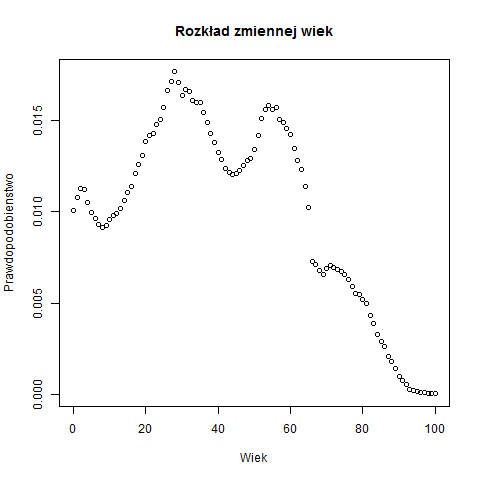
\includegraphics[width=\textwidth]{pictures/wiek.png}
    \caption{Rozkład prawdopodobieństwa zmiennej wiek}
    \label{fig:wiek}
  \end{subfigure}
  \hfill
  \begin{subfigure}[t]{0.45\textwidth}
    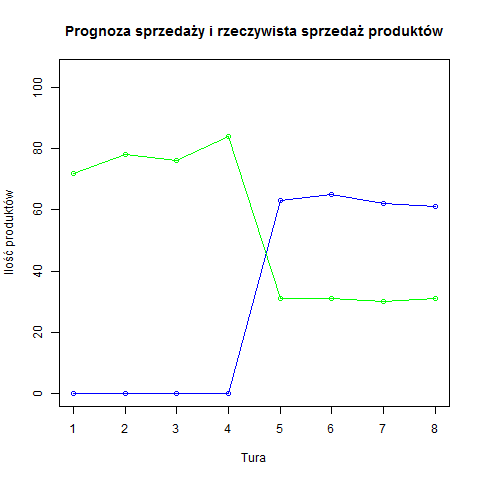
\includegraphics[width=\textwidth]{pictures/wyksztalcenie.png}
    \caption{Rozkład prawdopodobieństwa zmiennej wykształcenie}
    \label{fig:wyksztalcenie}
  \end{subfigure}
  \captionsetup{margin=10pt,font=small,labelfont=bf,width=.8\textwidth}
  \caption[Rozkłady zmiennych cech klasy konsument]{Rozkłady zmiennych cech klasy konsument \textit{Źródło:} opracowanie własne na podstawie danych Narodowego Spisu Ludności 2011, \cite{GUS2011}}\label{fig:wyksztalcenie}
\end{figure}
% --- figure --------------------------------------------------------


\subsubsection{Przedsiębiorstwo}

Zgodnie z założeniami określonymi w rozdziale 1, symulowane przedsiębiorstwo jest w istocie zbiorem niezależnych agentów. Zbiór ten należy w modelu do klasy \textit{firma}, przechowującej w macierzach instancje klas \textit{fabryka, magazyn, sklep}, jak zaprezentowano na diagramie \ref{firma}. W klasie \textit{firma} znajdują się także funkcje przynależne opisywanemu w strukturze modelu zarządowi, mające na celu koordynację działania przedsiębiorstwa. 

Warto zauważyć, że klasy te mają wiele wspólnych właściwości, z wyjątkami obecnymi w klasie \textit{sklep}. Wynika to z konieczności stworzenia funkcji symulujących sprzedaż oraz faktu, że sklepy mają dodatkowe zmienne przechowujące informacje o składzie towaru, klientach odwiedzających sklep w danej jednostce czasu $t$ oraz historii transakcji.  

% --- figure --------------------------------------------------------
\begin{figure}[hbt]
  \centering
\begin{tikzpicture} \label{firma}
\begin{class}[text width=7cm]{firma}{-1,0}
\attribute{fabryki : array}
\attribute{magazyny : array}
\attribute{sklepy : array}
\attribute{produkt : array}
\attribute{cena : array}
\operation{klienci\_w\_sklepach(self,swiat,tura)}
\operation{przypisz\_koszty(self,losowe,skala)}
\end{class}
\begin{class}[text width=6cm]{fabryka magazyn}{-5,-7}
\inherit{firma}
\attribute{nazwa : string}
\attribute{lokalizacja : array}
\attribute{oblozenie : integer}
\attribute{koszt : integer}
\attribute{efekt\_skali : integer}
\attribute{symbol : sympy.symbol}
\end{class}
\begin{class}[text width=7cm]{sklep}{2,-7}
\inherit{firma}
\attribute{nazwa : string}
\attribute{lokalizacja : array}
\attribute{oblozenie : integer}
\attribute{koszt : integer}
\attribute{efekt\_skali : integer}
\attribute{symbol:sympy.symbol}
\attribute{klienci : array}
\attribute{klienci\_historycznie : array}
\attribute{sklad : dictionary}
\attribute{sprzedaz : array}
\attribute{przewidywana\_sprzedaz:integer}
\operation{dostawa\_towaru(self, rynek, trasa, ilosc)}
\operation{sprzedaz\_w\_sklepie(self, towar)}
\end{class}
\end{tikzpicture}
  \captionsetup{margin=10pt,font=small,labelfont=bf,width=.8\textwidth}
  \caption[Diagram UML klasy firma, fabryka, magazyn oraz sklep]{Diagram UML klasy firma, fabryka, magazyn oraz sklep \textit{Źródło:} opracowanie własne}\label{UML:firma}
\end{figure}
% --- figure --------------------------------------------------------




\subsubsection{Produkt} \label{chapter:produkt}

Opierając się na stwierdzeniu \cite{Sagan2011}, który wskazuje na nurtu w dziedzinie modelowania strukturalnego zachowań klientów, które wykorzystywało zmienne marketingowe określające jakość produktu i ilość cech \footnote{Mowa o tzw. nurcie poznawczym albo nurcie teorii przetwarzania informacji - TPI}, zakładamy, że każdy produkt charakteryzuje się cechami wpływające na prawdopodobieństwo jego zakupu przez konsumentów które mogą być wyrażone ilościowo. 

Stąd produkt definiujemy przez zestaw wybranych cech które odróżniają go od produktów konkurencji, które mogą przyjąć formę skali ocen, zmiennych binarnych bądź zmiennych kategorycznych. \footnote{Ich istotność nie jest w tym momencie ważna, ponieważ nawet jeśli w zbiorze znajdzie się cecha mająca mały wpływ na decyzje konsumentów, zostanie ona wyeliminowana na etapie tworzenia modelu bądź drzewa klasyfikacyjnego ze względu brak istotności statystycznej współczynnika}, a klasa \textit{produkt} przechowujące jednowymiarową macierz z cechami produktu.

Warto odnotować, że w pracy przyjmujemy, że symulowanym produktem z branży FMCG jest piwo. Ten dość nieelegancki wybór motywowany jest głównie specyfiką produktu, która dobrze pasuje do wymagań stawianych przez model (szczególnie w aspekcie możliwości modelowania decyzji konsumenckich), wśród których są 

	\begin{itemize}
			\item wysoka sprzedaż i idący za tym wysoki obrót towaru w sklepach --- przeciętny polak pije 99 litrów piwa rocznie, co oznacza butelkę kupioną co mniej więcej drugi dzień, \footnote{Dzięki temu możemy założyć, że prawdopodobieństwo zakupu piwa przez klienta to nawet 50\% , a to z kolei gwarantuje odpowiednią ilość iteracji do przeprowadzenia analizy.} 
			\item produkt mają silne marki o ugruntowanych cecach i grupach docelowych --- reklamy piw zazwyczaj podkreślają w jakich okolicznościach i jaka grupa docelowa pije piwo, co powoduje, że występuje wysoka zależność pomiędzy charakterystyką demograficzną klienta a piwem które wybierze, \footnote{Idealnym przykładem jest Redd's, wybierany głównie przez kobiety. Innymi mogą być Grolsch wybierany przez ludzi zamożnych, kiedy Wojak trafia do najgorzej zarabiających}. 
			\item produkty mocno różnią się od siebie cechami --- w przeciwieństwie do mąki, rola jakości, smaku i właściwości piwa odgrywa znaczącą rolę dla klienta. Powoduje to, że piwo smakowe i pszeniczne będą trafiać do dwóch różnych grup klientów.
	\end{itemize}

% --- figure --------------------------------------------------------
\begin{table}[hbt]
  \centering
  \captionsetup{margin=10pt,font=small,labelfont=bf,width=.8\textwidth}
  \caption[Cechy charakteryzujące produkt w modelu]{Cechy charakteryzujące produkt w modelu. \textit{Źródło:} opracowanie własne.}
  \label{tab:cechyproduktu}
\vspace*{2ex}
\begin{tabular}{llll}
\hline
Cecha      & Rodzaj zmiennej  & Skala & Opis                                                                                                        \\ \hline
Cena       & Liczba naturalna & 1-5   & Relatywna cena produktu w odniesieniu do rynku                                                              \\
Smak       & Liczba naturalna & 1-5   & Relatywna jakość smaku produktu w odniesieniu do rynku                                                      \\
Opakowanie & Liczba naturalna & 1-5   & Relatywna atrakcyjność opakowania produktu w odniesieniu do rynku                                           \\
Premium    & Zmienna binarna  & 0-1   & Czy produkt jest postrzegany jako marka premium (tj. kierowany do najbardziej zamożnych klientów) na rynku? \\
Budżetowy  & Zmienna binarna  & 0-1   & Czy produkt jest postrzegany jako marka budżetowa (tj. kierowany do najmniej zamożnych klientów) na rynku?  \\
Lager      & Zmienna binarna  & 0-1   & Czy produkt należy do piw typu lager?                                                                       \\
Smakowe    & Zmienna binarna  & 0-1   & Czy produkt należy do piw smakowych?                                                                        \\
Marketing  & Liczba naturalna & 0-5   & Wysokość nakładów na marketing marki                                                                        \\ \hline
\end{tabular}
\end{table}
% --- figure --------------------------------------------------------

\subsubsection{Konkurencja}
 
W założeniach przyjmujemy, że konkurencja jest pasywna - tj. nie podejmuje działań ani decyzji w trakcie trwania symulacji. Wynika to z odmiennego celu badania, którym jest analiza działania algorytmów optymalizacyjnych. Nagłe zmiany sprzedaży spowodowane np. obniżeniem ceny przez konkurencję spowodowałyby wątpliwości interpretacyjne i są zbędne. Konkurencja jest za to potrzebna do stworzenia alternatywnych dla symulowanego produktu, o odmiennych cechach i przyciągających klientów o specyficznych charakterystykach, i jej rola ogranicza się do wprowadzenia go na rynek.

\subsubsection{Trasy}

Klasa \textit{trasy} przechowuje wszystkie możliwe kombinacje łańcuchów dostaw, składające się z instacji klas \textit{fabryka}, \textit{magazyn}, \textit{sklep} oraz \textit{scieżek} pomiędzy nimi \footnote{Jako ścieżkę rozumiemy sekwencję punktów z drogami, jakie trzeba przebyć od fabryki do magazynu i od magazynu do skepu}. W przypadku złożonych grafów (czyli sytuacji, kiedy przedsiębiorstwo składa się z wielu jednostek) ilość kombinacji może uniemożliwić swodobne przetwarzanie klasy w pamięci komputera, jednak w takim wypadku można predefiniować zbiór możliwych łańcuchów, spośród których model będzie wybierał najbardziej optymalne trasy. 

Dla każdej z tras, poza informacjami o jednostkach wchodzących w skład przedsiębiorstwa, przechowujemy także informację o \textit{scieżkach} pomiędzy jednostkami. Wynika to z faktu, że transporty pomiędzy poszczególnymi jednostkami także mogą doświadczać efektów skali, \footnote{Przykładowo, pod kątem kosztów na produkt, transport 100 produktów może być bardziej opłacalny niż 10  ze względu na rozłożenie kosztów stałych na większą ilość produktów} a długość ścieżki bezpośrednio wpływa na koszt łańcucha - koszt wzrasta w stosunku do długości ścieżki.

\subsection{Symulowanie decyzji konsumenckich} \label{chapter:customerresearch}

Jak wskazano na diagramie \ref{fig:struktura}, podczas wizyty każdego z wirtualnych konsumentów w sklepie symulujemy jego decyzję co do zakupu towaru. W tej części chcemy, aby decyzje konsumentów w modelu jak najbardziej przypominały decyzje klientów w analogicznych sytuacjach w świecie rzeczywistym. \footnote{Warto odnotować, że to nie jest to samo co późniejsze przewidywanie "prognozowanej sprzedaży"} 

Opierając się na \cite{Sagan2011}, wiemy, że jesteśmy w stanie zdefiniować kluczowe cechy konsumenta i cechy marketingowe produktu jako zbiór zmiennych ilościowych. Stąd, w grze eksperymentalnej przeprowadzonej na potrzeby pracy \footnote{Gra dostępna jest pod adresem http://serwer1418288.home.pl/test/piwo/zapisy.php}, poproszono uczestników o stwierdzenie, jakie produkty z dostępnej listy kupi klient o charakterystyce wylosowanej przez program. Po odpowiedzi udzielonej przez gracza, predefiniowane, jakościowe cechy produktu były transponowane na wartości liczbowe \footnote{Na przykład, piwo Grolsh jest drogie, klasy premium i jest lager, stąd otrzyma zapis [5,1,1], a tani smakowy Redd's [3,0,0].} i wraz z ilościowymi cechami klienta oraz zmienną binarną przechowującą informacje \textit{kupił/niekupił} zapisywany na serwerze SQL. 

W programie dane te służą do budowy drzewa klasyfikacyjnego, które - ponieważ dane liczbiowe są w identycznej formie- dla każdej kwerendy o klienta i produkt zwraca prawdopodobieństwo zakupu. Stąd, dla każdego agenta możemy zbudować listę prawdopodobieństw zakupu każdego z towarów dostępnego na rynku, i w ten sposób losowaniem symulować decyzje konsumenckie. To podejście gwarantuje wysokie podobieństwo z wyborami realnych konsumentów ponieważ

	\begin{itemize}
		\item ze względu na wysoką ilość rekordów jest duża szansa, że istnieje zapis o decyzjach klienta o bardzo podobnej charakterystyce
		\item baza danych jest generowania przez decyzje ludzkie, zapewniając wysoką zgodność z analogicznymi wyborami w świecie rzeczywistym
		\item wybór drzewa klasyfikacyjnego  jako metody i wysoki $n$ rekordówpozwala na bardzo pożądany w tej sytuacji \textit{overfit}, który jak opisuje \cite{James2013} powoduje, że dostajemy bardzo dokładne odwzorowanie zbioru uczącego. 
	\end{itemize}

% --- chapter ---------------------------------------------------------
\clearpage
\section{Efekty działania algorytmu optymalizacyjnego}

\subsection{Założenia modelu}

Weryfikacja działania algorytmu odbywać się będzie w modelu opisanym w rozdziale \ref{chapter:model}, w oparciu o losowo wygenerowane środowisko działania modelu (\textit{świat i rynek}), których właściwości zostały opisane w w tabeli \ref{tab:zalozenia}. Mapy powstałego w ten sposób środowiska zostały przedstaiwone na wykresach \ref{symulowanamapa} i \ref{symulowanaludnosc}, a symulowane przedsiębiorstwo zostało przedstawione w postaci grafu na wykresie \ref{fig:prostygraf}.

\begin{table}[hbt] 
  \centering
  \captionsetup{margin=10pt,font=small,labelfont=bf,width=.8\textwidth}
  \caption[Właściwości generowanego świata]{Założenia generowanego świata. \textit{Źródło:} opracowanie własne.}
  \label{tab:zalozenia}
\vspace*{2ex}
  \begin{tabular}{lccc}
    Właściwość        & Założenie \\ \hline
    Populacja & $2 500$\\
    Wymiar $x$ & $60$\\
    Wymiar $y$ & $60$\\ 
    Udział dróg & $0.3$\\ 
    Gęstość zakrętów dróg & $0.05$\\  
    Udział budynków mieszkalnych & $0.6$\\  
    Udział biurowców \footnote{Biurowce są dla konsumentów miejscem pracy, do których podróżują codziennie} & $0.2$\\  
    Udział przestrzeni komercyjnej \footnote{Przestrzeń komercyjna to miejsca, w którym można założyć sklep, fabrykę bądź magazyn, tak więc razem tworzą zbiór miejsc gdzie przedsiębiorstwo może losowo wygenerować swoją jednostkę}& $0.2$\\  \hline
    Ilość fabryk & 2\\ 
    Ilość magazynów & 2\\ 
    Ilość ilość sklepów & 4\\ 
    Cena produktu & 7\\ 
  \end{tabular}
\end{table}

\begin{figure}[hbt]
  \centering
  \begin{subfigure}[t]{0.45\textwidth}
    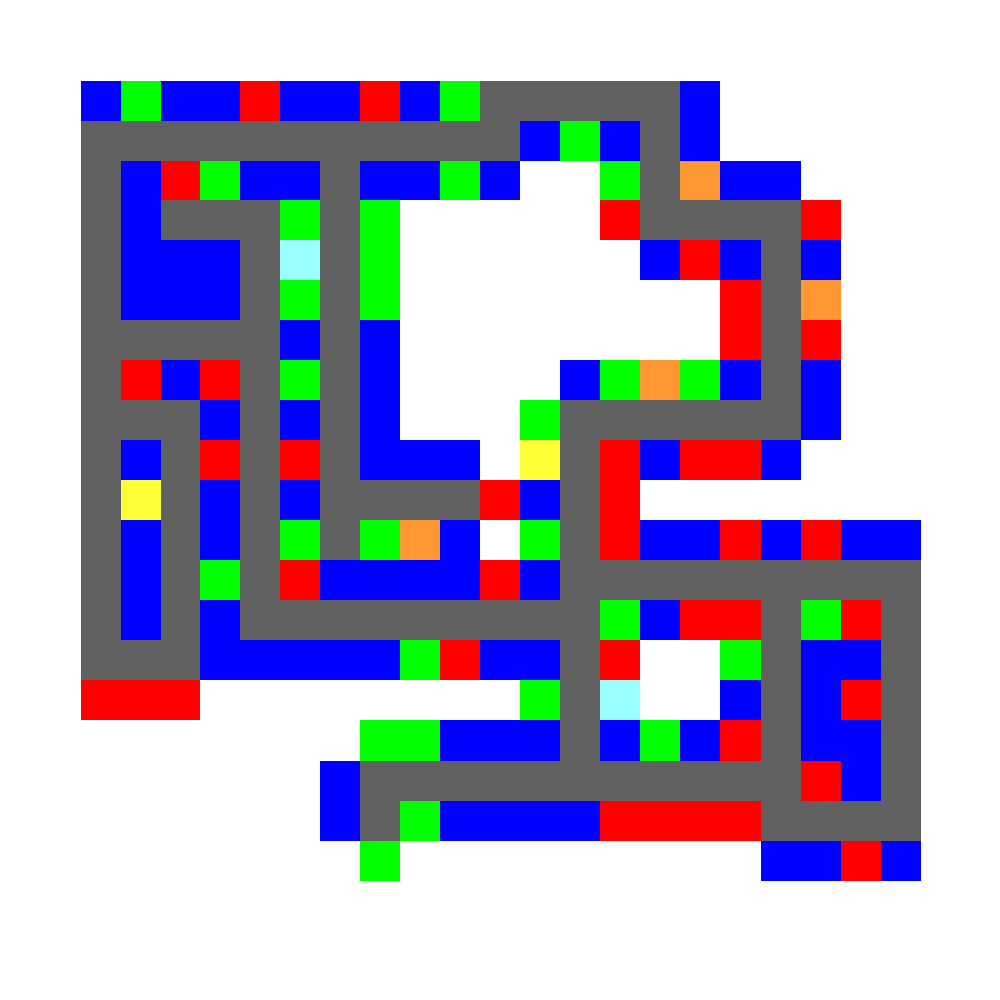
\includegraphics[width=\textwidth]{../mapy/typy.png}
    \caption{Mapa typów lokacji na mapie}
    \label{symulowanamapa}
  \end{subfigure}
  \hfill
  \begin{subfigure}[t]{0.45\textwidth}
    
\includegraphics[width=\textwidth]{../mapy/ludnosc.png}
    \caption{Histogram występowania konsumentów na mapie.}
    \label{symulowanaludnosc}
  \end{subfigure}
  
  \captionsetup{margin=10pt,font=small,labelfont=bf,width=.8\textwidth}

  \caption[Krótka nazwa II]{Mapa wygenerowanych macierzy lokalizacji w modelu}\label{fig:xxx}
\end{figure}

\paragraph{Konsumenci}\mbox{}\\
Cechy konsumentów zostały wygenerowane zgodnie z rozkładami zawartymi w Narodowym Spisie Ludności (\cite{GUS2011}) oraz XI Ogólnopolskim Badaniu Wynagrodzień \cite{Sedlak2013} w celu zapewnienia spójności z rzeczywistą strukturą społeczną. Histogramy cech klientów w modelu zostały zaprezentowane na wykresie \ref{ludnosc}. 

Jak zostało opisane w rozdziale \ref{chapter:konsumenci}, cechy klientów wpływają na ich decyzji konsumenckie i wybór produktów w sklepie. Dlatego profil klienta konsumującego symulowany produkt (zob. tabela \ref{tab:produkty}) będzie dystynktywny, tak jak w normalnych warunkach rynków różne marki przyciągają klientów o różnych profilach i cechach demograficznych. Właściwość tą wykorzystujemy do modelowania predyktywnego prawdopodobieństwa zakupu przy danej charakterystyce klienta w czasie $t+1$. Porównanie rozkładów cech wszystkich klientów i konsumentów marki zaprezentowano na wykresie \ref{profile}.

\begin{figure}[hbt]
  \centering
    
\includegraphics[width=\textwidth]{pictures/ludnosc.png}
  \captionsetup{margin=10pt,font=small,labelfont=bf,width=.8\textwidth}
  \caption[Histogramy cech agentów]{Histogramy cech agentów. \textit{Źródło:} opracowanie własne}\label{ludnosc}
\end{figure}

\begin{figure}[hbt]
  \centering
    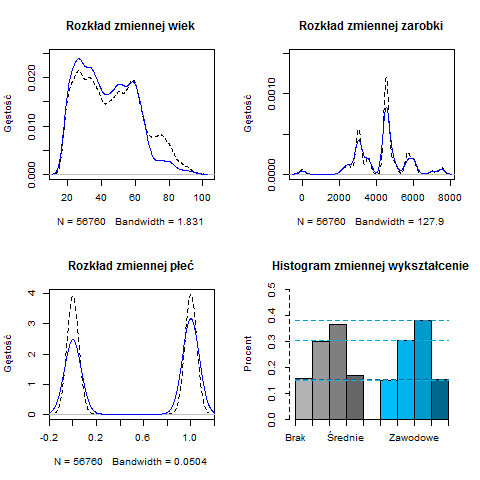
\includegraphics[width=\textwidth]{pictures/profile_klientow.png}
  \captionsetup{margin=10pt,font=small,labelfont=bf,width=.8\textwidth}
  \caption[Cechy konsumentów marki w porównaniu do wszystkich agentów]{Cechy konsumentów marki w porównaniu do wszystkich agentów. Na czarno zaznaczone dane dla wszystkich klientów, na niebiesko --- dla klientów marki. \textit{Źródło:} opracowanie własne}\label{profile}
\end{figure}


\paragraph{Przedsiębiorstwo}\mbox{}\\
Symulowane przedsiębiorstwo, zdefiniowane jak w rozdziale \ref{chapter:zadanie}, składa się z zaprezentowanej w tabeli \ref{tab:zalozenia} ilości jednostek --- 2 fabryk, 2 magazynów i 4 sklepów, które wspólnie tworzą  $2\choose 1 $ $ \times $ $2\choose 1 $ $ \times $ $4\choose 1 $ = 16 możliwych ścieżek. Lokacje poszczególnych jednostek zostały zaprezentowane na rysunku \ref{mapafirma}.

Każdy z $j$ elementów przedsiębiorstwa oraz krawędzie $d$ je łączące powiązane jest z funkcją kosztu $f_j$, które w celu symulacji efektów skali są nieliniowe. Dla fabryk, magazynów i sklepów zakładamy ujemne korzyści skali, podczas gdy dla transportu na krawędziach --- dodatnie. Dokładne funkcje kosztów wykorzystane w modelu opisane są w tabelli \ref{tab:funkcje_kosztow}. 

\begin{table}[hbt]
  \centering
  \captionsetup{margin=10pt,font=small,labelfont=bf,width=.8\textwidth}
  \caption[Założone w modelu funkcje kosztów]{Założone w modelu funkcje kosztów. \textit{Źródło:} opracowanie własne.}
  \label{tab:funkcje_kosztow}
\vspace*{2ex}
  \begin{tabular}{lccc}
    Jednostka        & Symbol & Funkcja kosztu \footnote{$x_j$ definiujemy jako wolumen przechodzący przez dany element grafu $f \in S$}\\ \hline
    Fabryka    & $fa \in FA$   &    $f_{fa} =  1.3 \times x_{fa} ^{1.03}$ \\
    Magazyn & $ma \in MA$  & $ f_{ma} = 1.2 \times x_{ma} ^{1.05}$\\
    Sklep & $sk \in SK$ & $f_{sk} = 1.1 \times x_{sk} ^{1.07}$\\ 
    Droga (krawędź ) & $ d \in D \footnote{$l_d$ jest długością krawędzi, liczoną jako ilość punktów które należy przebyć od jej początku do końca}$ & $ f_{d} = 0.005 \times l_d \times x_{d} ^{0.95}  $ \\ \hline
  \end{tabular}
\end{table}


\begin{figure}[hbt]
  \centering
\begin{center}
\begin{tikzpicture}
   % Draw all levels
  \draw[level] (0,-1) -- node[above] {fabryka  $fa_1$}  (2,-1);
  \draw[level] (0,1) -- node[above] {fabryka  $fa_1$}   (2,1);
  \draw[connect] (2,1)  -- (3,1);
  \draw[connect] (2,1)  -- (3,-1);
  \draw[connect] (2,-1)  -- (3,-1);
  \draw[connect] (2,-1)  -- (3,1);
  \draw[level]   (3,1)  -- node[above] {magazyn  $ma_1$}  (5,1);
  \draw[level]   (3,-1)  -- node[above] {magazyn  $ma_1$}  (5,-1);
  \draw[level]   (6,1.5)  -- node[above] {sklep $sk_1$}   (8,1.5); 
  \draw[level]   (6,0.5)  -- node[above] {sklep $sk_2$} (8,0.5);
  \draw[level]   (6,-0.5)  -- node[above] {sklep $sk_2$} (8,-0.5);
  \draw[level]   (6,-1.5)  -- node[above] {sklep $sk_2$} (8,-1.5);
  \draw[connect] (5,1)    -- (6,1.5)  (5,1) -- (6,0.5) (5,1) -- (6,-0.5) (5,1) -- (6,-1.5);
 \draw[connect] (5,-1)    -- (6,1.5)  (5,-1) -- (6,0.5) (5,-1) -- (6,-0.5) (5,-1) -- (6,-1.5);
  % Draw labels
  \node[label] at (1,3)  {\textit{Fabryki}};
  \node[label] at (4,3)  {\textit{Magazyny}};
  \node[label] at (7.5,3)  {\textit{Sklepy}};
  % Draw annotations
\end{tikzpicture}
\end{center}
  \captionsetup{margin=10pt,font=small,labelfont=bf,width=.8\textwidth}
  \caption[Modelowane przedsiębiorstwo przedstawione jako graf kierunkowy]{Modelowane przedsiębiorstwo przedstawione jako graf kierunkowy  \textit{Źródło:} opracowanie własne}\label{fig:prostygraf}
\end{figure}



\begin{figure}[hbt]
  \centering
    
\includegraphics[width=\textwidth]{../mapy/firma.png}
  \captionsetup{margin=10pt,font=small,labelfont=bf,width=.8\textwidth}
  \caption[Krótka nazwa X]{Mapa z zaznaczonymi jednostkami przedsiębiorstwa. \textit{Źródło:} opracowanie własne}\label{mapafirma}
\end{figure}

\paragraph{Produkty}\mbox{}\\
W modelu zakładamy, że na rynku obecnych jest 7 marek piwa, z których jedno należy do symulowanego przez nas przedsiębiorstwa (produkt o nazwie \textbf{Symulowane}). Jak opisano w rozdziale \ref{chapter:produkt}, każde z piw zdefiniowane jest 7 zmiennymi marketingowymi, których cechy produktów zostały zaprezentowane zostały w tabeli \ref{tab:produkty}. Wyniki sprzedaży poszczególnych marek w jednostkach czasu $t$ zaprezentowane są na wykresie \ref{fig:sprzedaz_marek}.

Zauważmy w tabeli \ref{tab:produkty}, że piwo należące do symulowanego przez nas przedsiębiorstwa należy do jednych z najtańszych piw na rynku, jest piwem smakowym o przeciętnych walorach smakowych, ale za to intensywnych nakładach na marketing i dużej uwadze poświęconej projektowaniu opakowania. Skonfrontowanie tego z profilem klienta widocznym na wykresie \ref{profile} pozwala zrozumieć, dlaczego nabywcy naszego piwa należą do grupy gorzej sytuowanych finansowo, raczej młodszych \footnote{Wynika to z połączenia faktów, że młode osoby mniej zarabiają, oraz piwa smakowe nie są zbyt popularne wsród starszych roczników}, z dominującą grupą kobiet. Profil wykształcenia nie różni się znacząco od przeciętnej, z delikatnie mniejszym udziałem klientów o wyższym wykształceniu.

\begin{figure}[hbt]
  \centering
    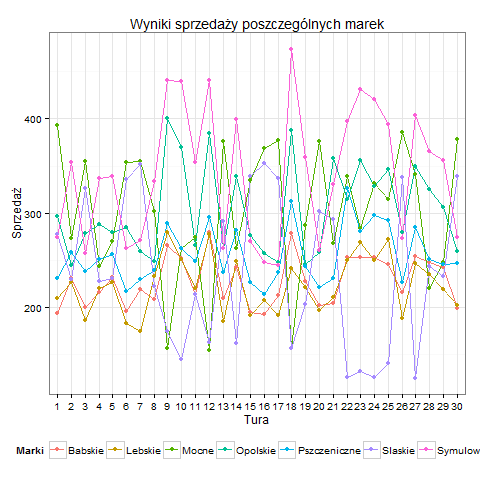
\includegraphics[width=\textwidth]{pictures/sprzedaz_marek.png}
  \captionsetup{margin=10pt,font=small,labelfont=bf,width=.8\textwidth}
  \caption[Statystyki sprzedaży marek symulowanych w modelu]{Statystyki sprzedaży marek symulowanych w modelu. \textit{Źródło:} opracowanie własne}\label{fig:sprzedaz_marek}
\end{figure}


\begin{table}[hbt] 
  \centering
  \captionsetup{margin=10pt,font=small,labelfont=bf,width=.8\textwidth}
  \caption[Cechy symulowanych produktów]{Cechy symulowanych produktów. \footnote{Cechy określone przez nazwy binarne zostały opisane skrótem: P --- premium, B --- budżetowe, L --- lager, S --- smakowe} \footnote{Opis poszczególnych cech zawarty jest w tabeli \ref{tab:cechyprodukty}}\textit{Źródło:} opracowanie własne.}
  \label{tab:produkty}
\vspace*{2ex}
  \begin{tabular}{rcccccccc}
  \hline
 & Cena & Smak & Opakowanie & P & B & L & S & Marketing \\ 
  \hline
\textbf{Symulowane} &   1 &   3 &   5 &   0 &   0 &   0 &   1 &   4 \\ 
  Slaskie &   4 &   4 &   2 &   1 &   0 &   1 &   0 &   4 \\ 
  Lebskie &   4 &   2 &   2 &   1 &   0 &   0 &   1 &   5 \\ 
  Babskie &   4 &   3 &   5 &   0 &   1 &   0 &   1 &   5 \\ 
  Pszczeniczne &   2 &   2 &   2 &   0 &   0 &   0 &   1 &   2 \\ 
  Opolskie &   4 &   3 &   5 &   0 &   0 &   0 &   1 &   4 \\ 
  Mocne &   4 &   2 &   2 &   1 &   0 &   1 &   0 &   3 \\ 
   \hline
\end{tabular}
\end{table} 



\subsection{Przewidywanie decyzji konsumentów}

Przewidywanie decyzji konsumentów odbywa się zgodnie z założeniami przedstawionymi w rozdziale \ref{chapter:statistical}. \footnote{W modelu stosowane jest pewne uproszczenie podczas prognozowania ilości klientów w sklepie w $t+1$. Ponieważ wizyta klienta w sklepie jest w modelu zdarzeniem losowym (losuje się jedna z czterech lokalizacji docelowych), a model nie symuluje efektów zewnętrznych jak pogoda czy dzień tygodnia, do przewidywania liczby klientów odwiedzających sklep w chwili $t+1$ stosowana jest średnia. Brak jest bowiem zmiennych objaśniających które mogłyby zostać wykorzystane w modelu, jednak ich wprowadzenie dodawałoby niepotrzebną złożoność do modelu, a zastosowane uproszczenie nie ma wpływu na badanie wyników działania algorytmu}. Kolejne kroki prognozowania sprzedaży w każdym ze sklepów w czasie $t+1$ to 

\begin{enumerate}
	\item Na podstawie historii transakcji obliczamy średnią ilość klientów $n$ odwiedzających sklep w jednostce czasu $t$
	\item Na podstawie historii cech klientów kupujących produkt, obliczamy prawdopodobieństwo warunkowe wystąpienia wszystkich zestawów cech, i losujemy cechy dla $n$ klientów w $t+1$ 
	\item Dla każdego z tak otrzymanych klientów na podstawie przeszłej historii wyborów klientów, wykorzystując metodę regresji logistycznej bądź klasyfikacji k-means, obliczamy 			prawdopodobieństwo zakupu produktu symulowanej firmy
	\item Kroki 1-3 powtarzamy założoną ilość razy \footnote{W modelu przyjmujemy 3 iteracje} i obliczamy średnią z trzech obserwacji
\end{enumerate} 

Analizując wyniki prognozowania, przedstawione na wykresach na wykresach \ref{fig:prognozy_porowniania} możemy zobserwować różnicę w skuteczności prognoz obu stosowanych metod --- \textit{regresji logistycznej} oraz \textit{k-nearest neighbours}. Chociaż współczynnik determinacji $R^2$ jest wyższy dla metody regresji logistycznej ($R_{lg}^2 = 0,7912$) niż dla K-nearest neighbours ($R_{kn}^2 = 0,7591$), to najcenniejszą cechą regresji jest, że nie przeszacowuje sprzedaży tak jak to robi K-nearest neighbours. Nadmierny optymizm metody K-nearest neighbours powoduje, że zamawia się produkty o których wiemy, że nie zostaną sprzedane, ponosząc niepotrzebne koszty produkcji i transportu (zob. wykres \ref{fig:przychody_koszty}. 

Wynika to z faktu, że K-nearest neighbours dla współczynnika $k=3$ ma większe trudności z jednoznacznym określeniem klasy przewidywanej zmiennej \footnote{Warto przypomnieć, że w tym momencie modelujemy to, czy dany klient będzie w klasie 0 (\textit{nie kupił}) czy 1 (\textit{kupił})} niż regresja logistyczna, jak możemy to zaobserwować na wykresie \ref{fig:rozklad_lg_kn}. Regresja logistyczna jest o wiele bardziej skłonna to przyporządkowania niskiego prawdopodobieństwa zakupu, jednak z większą pewnością określa klientów którzy kupią produkt. Tymczasem, k-nearest neighbours często wskazuje wartość prawdopodobieństwa w środku przedziału $(0,1)$, dając odpowiedź niejednoznaczną. Możliwe, że manipulacja współczynnikiem $k$ wpłynęła by na zachowanie metody, jednak w przypadku modelu za bardziej skuteczną będziemy uważać metodę regresji logistycznej. 

\begin{figure}[hbt]
  \centering

  \begin{subfigure}[t]{0.45\textwidth}
    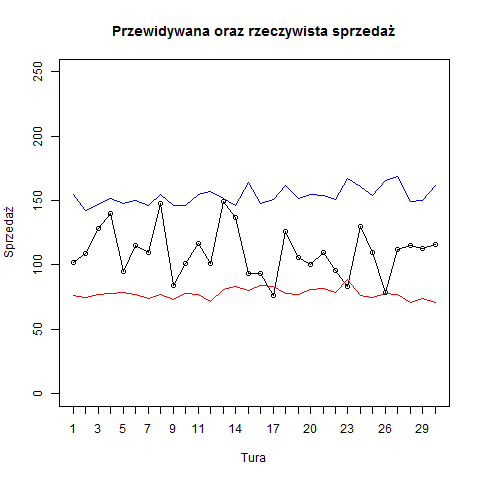
\includegraphics[width=\textwidth]{pictures/prognozy_lg_kn.png}
  \end{subfigure}
  \captionsetup{margin=10pt,font=small,labelfont=bf,width=.8\textwidth}

  \caption[Przewidywana i realna sprzedaż w modelu]{Przewidywana i realna sprzedaż w modelu. Prognoza metodą regresji logistycznej zaznaczona na niebiesko, metoda K-neareast neighbours --- czerwono \textit{Źródło:} opracowanie własne}\label{fig:lg_kn}
\end{figure}

\begin{figure}[hbt]
  \centering

  \begin{subfigure}[t]{0.45\textwidth}
    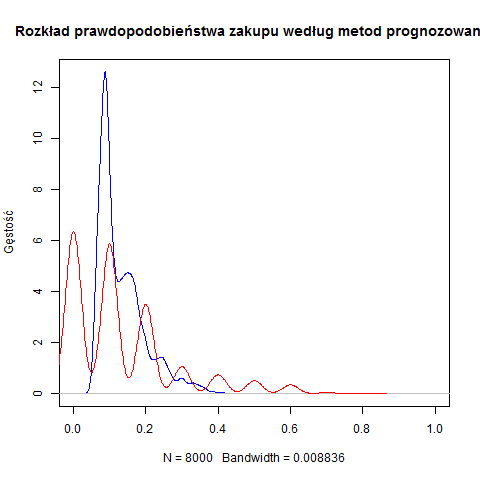
\includegraphics[width=\textwidth]{pictures/rozklad_prognoz}
  \end{subfigure}
  \captionsetup{margin=10pt,font=small,labelfont=bf,width=.8\textwidth}

  \caption[Rozkład prawdopodobieństwa zakupu w prognozach]{Rozkład prawdopodobieństwa zakupu w prognozach według metod prognoz. Prognoza metodą regresji logistycznej zaznaczona na niebiesko, metoda K-neareast neighbours --- czerwono \textit{Źródło:} opracowanie własne}\label{fig:rozklad_lg_kn}
\end{figure}

\subsection{Wpływ działania algorytmu na działanie przedsiębiorstwo} \label{chapter:wyniki}

Na początku symulacji przez 20 jednostek czasu $t$, w celu uzyskania punktu odniesienia, przedsiębiorstwo podejmuje decyzje na podstawie predefiniowanych zasad opisanych w rozdziale \ref{chapter:koncepcja}, czyli 

	\begin{itemize}
		\item towar zamawiamy jest zawsze z najbliższego magazynu
		\item ilość zamówionego towaru do każdego ze sklepów równa jest sprzedaży $t_0$ \footnote{Gdzie $t_0$ to runda próbna, która ma na celu sprawdzenie popytu na rynku i nie jest zapisywana do wyników firmy. Jej wdrożenie ma na celu odwzierciedlenie w modelu wiedzy powszechnej o rynku, tj. przedsiębiorcy wiedzą ile mogą sprzedać na podstawie tego, co sprzedawali w niedalekiej przeszłości albo na podstawie raportów rynkowych}
	\end{itemize}

Po 20 jednostkach czasu na podstawie dotychczasowej historii transakcji inicjalizowane są modele regresji logistycznej oraz k-nearest neighbours, które przez następne 10 jednostek czasu $t$ słuzą do prognozowania sprzedaży w każdym ze sklepów w $t+1$. Zgodnie z przyjętymi w rozdziale \ref{chapter:zadanie}, wiedza o sprzedaży w każdym ze sklepów w $t+1$ pozwala nam, po odpowiednich przekształceniach, zbudować algorytm optymalizujący procesy produkcyjno-logistyczne, przede wszystkim pod kątem alokacji wolumenów produkcji i tras dostaw pomiędzy poszczególne jednostki przedsiębiorstwa. 

\paragraph{Alokacje na trasach dostaw (ścieżkach)}\mbox{}\\

W rezultacie działania modelu otrzymujemy wektor $A$, który dla każdego elementu zbioru $w \in W$ (zob. rozdział \ref{chapter:zadanie}) zawiera optymalny \footnote{Zastrzeżenia wobec optymalności alokacji sugerowanych przez algorytm znalazły się w rozdziale \ref{chapter:algorytm}} wolumen dostaw w $t+1$. Wektory otrzymane w toku działania modelu zostały zaprezentowane na wykresie \ref{fig:sciezki}.

Analiza wykresu wyraźnie pokazuje, że przedsiębiorstwo sterowane przez algorytm jest o wiele bardziej elastyczne co do wyboru ścieżek, na co wskazuje rosnąca po $t=20$ wariancja alokacji. Ponadto, algorytm potrafi dostarczyć towar do sklepu z wielu źródeł. Biorąc pod uwagę, że funkcje kosztów są nieliniowe a we wszystkich jednostkach firmy występują negatywne efekty skali, pozwala to znaczące ograniczenie kosztów. 

To o tyle ważna obserwacja, że w praktyce biznesowej podobne metody ograniczenia kosztów nie są szeroko stosowane. Wręcz przeciwnie, często pracownicy firmy podczas składania zamówień podejmują decyzje, które lokalnie wydają się im być najlepsze (np. zamawianie z najbliższego magazynu), ale z punktu widzenia całego systemu nie są optymalne. Zastosowanie podobnych do opisywanego algorytmów może przynieść znaczące oszczędności w przedsiębiorstwach. 

\begin{figure}[hbt]
  \centering

  \begin{subfigure}[t]{0.45\textwidth}
    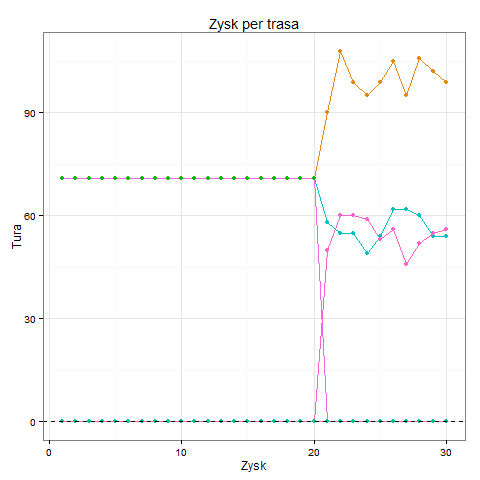
\includegraphics[width=\textwidth]{pictures/trasy.png}
  \end{subfigure}

  \captionsetup{margin=10pt,font=small,labelfont=bf,width=.8\textwidth}

  \caption[Alokacje wolumenów dostaw wśród możliwych ścieżek]{Alokacje wolumenów dostaw wśród możliwych ścieżek. Przerywana liniia oznacza inicjalizację działania modelu. \textit{Źródło:} opracowanie własne}\label{fig:sciezki}
\end{figure}


\paragraph{Przychody i koszty} \mbox{}\\

Obserwacja przychodów, kosztów i zysków przedsiębiorstwa w modelu, przedstawione odpowiednio na wykresach \ref{fig:zysk} oraz \ref{fig:przychod_koszt}, pozwala zauważyć, że działanie algorytmu wpłynęło \textit{in plus} na wyniki firmy. Warto odnotować, że przedsiębiorstwo w początkowych turach miało stabiline koszty, które jak wspomniano w rozdziale \ref{chapter:koncepcja}, starano się minimalizować, zamawiając towary tylko z najbliższego magazynu. 

Chociaż jest to racjonalna strategia, nie była jednak skuteczna w obliczu dużej zmienności ilości klientów w sklepach, którą można zaobserwować na wykresie \ref{fig:lg_kn}, była wysoce nieskuteczna --- zyskowne okresy przeplatały się z nierentownym. Straty w niektórych okresach wynikały przede wszystkim z niepotrzebnie wysokich kosztów zamówień oraz nieumiejętności dostosowania się do wysokiej zmienności wolumenu sprzedaży, co wymagałało większej elastyczności w zamówieniach. Model, jak zaobserwowano w \ref{chapter:wyniki} jest bardziej elastyczny, dzięki czemu mógł lepiej dostosowywać się do popytu i odnotowywać zysk w każdej turze. 

Dodatkowo, gdyby zmienność nie była wywołana losowo, jak w modelu, ale zależna od serii czynników (pogoda, dzień tygodnia, etc), możliwe byłoby stworzenie modelu który wyłapywałby takie zmiany w tendencjach i potrafiłby dostosować do nich produkcję. Dobrym przykładem skuteczności takiego algorytmu byłby model przewidujący sprzedaż lodów, który przy prognozie dobrej pogody zwiększałby zapasy, a przy ochłodzeniach redukował produkcję. Zazwyczaj takie procesy koordynowane są przez ludzi, jednak duża ilość zmiennych oraz możliwa ich heterogeniczność (różna pogoda w różnych częściach Polski) powoduje, że pewne prognozy są zbyt złożone żebyśmy mogli je przewidywać z wysoką dokładnością bez metod matematycznych. 

\begin{figure}[hbt]
  \centering
  \begin{subfigure}[t]{0.45\textwidth}
    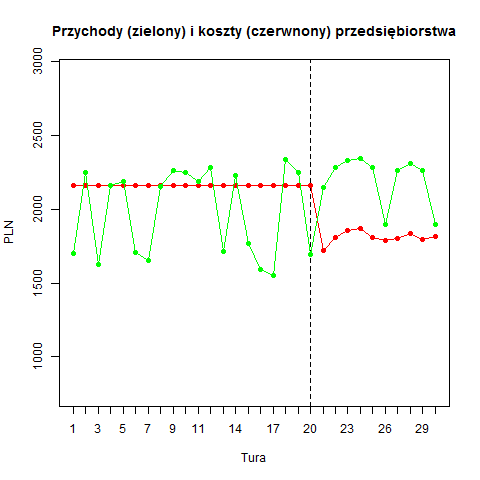
\includegraphics[width=\textwidth]{pictures/przychody_koszty_lm.png}
    \caption{Przychody i koszty symulowane przedsiębiorstwa w symulacji z metodą prognozowania regresji logistycznej}
    \label{fig:przychod_koszt}
  \end{subfigure}
  \hfill
  \begin{subfigure}[t]{0.45\textwidth}

    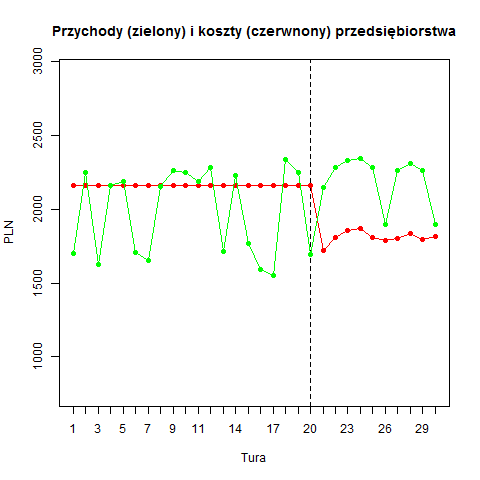
\includegraphics[width=\textwidth]{pictures/przcyhody_koszty_kn.png}
    \caption{Przychody i koszty symulowane przedsiębiorstwa w symulacji z metodą prognozowania k-nearest neighbours}
    \label{fig:zysk}
  \end{subfigure}
  
  \captionsetup{margin=10pt,font=small,labelfont=bf,width=.8\textwidth}

  \caption[Wyniki finansowe symulowanego przedsiębiorstwa]{Wyniki finansowe symulowanego przedsiębiorstwa. Przerywana linia oznacza inicjalizację algorytmu. \textit{Źródło:} opracowanie własne}\label{fig:wynikifin}
\end{figure}

\begin{figure}[hbt]
  \centering
  \begin{subfigure}[t]{0.45\textwidth}
    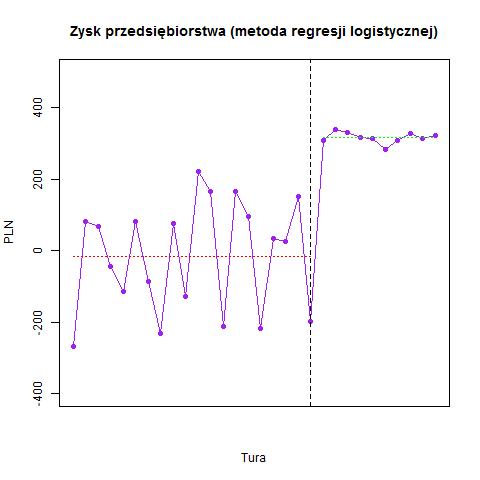
\includegraphics[width=\textwidth]{pictures/zysk_lm.png}
    \caption{Zysk symulowanego przedsiębiorstwa, z zaznaczonymi średnimi zyskami przed i po inicjalizacji algorytmu}
    \label{fig:przychod_koszt}
  \end{subfigure}
  \hfill
  \begin{subfigure}[t]{0.45\textwidth}

    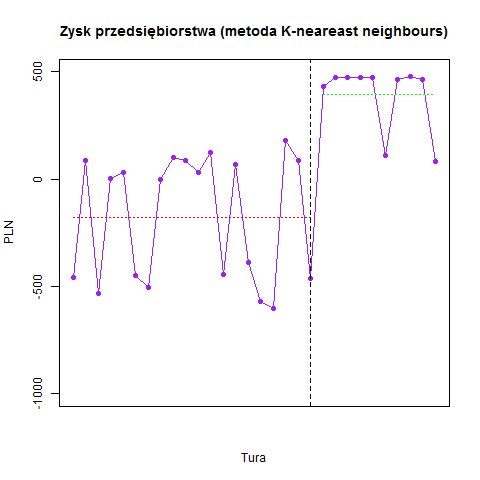
\includegraphics[width=\textwidth]{pictures/zysk_km.png}
    \caption{Zysk symulowanego przedsiębiorstwa w symulacji z metodą prognozowania regresji logistycznej, z zaznaczonymi średnimi zyskami przed i po inicjalizacji algorytmu}
    \label{fig:zysk}
  \end{subfigure}
  
  \captionsetup{margin=10pt,font=small,labelfont=bf,width=.8\textwidth}

  \caption[Zysk symulowanego przedsiębiorstwa]{Zysk symulowanego przedsiębiorstwa, z zaznaczonymi średnimi zyskami przed i po inicjalizacji algorytmu. Przerywana linia oznacza inicjalizację algorytmu. \textit{Źródło:} opracowanie własne}\label{fig:wynikifin}
\end{figure}


% --- appendices ------------------------------------------------------
\appendix

% --- bibliography ----------------------------------------------------
\clearpage
\bibliographystyle{agsm}
\bibliography{refs}

% --- abstract --------------------------------------------------------
\clearpage
\addcontentsline{toc}{section}{Lista tablic}
\listoftables

% --- abstract --------------------------------------------------------
\clearpage
\addcontentsline{toc}{section}{Lista rysunków}
\listoffigures



% --- abstract --------------------------------------------------------
\clearpage
\addcontentsline{toc}{section}{Streszczenie}
\section*{Streszczenie}



\end{document}

